\documentclass{article}
\usepackage{graphicx} 
\usepackage{caption}
\usepackage{geometry}
 \geometry{
 a4paper,
 total={170mm,257mm},
 left=20mm,
 top=20mm,
 }
 
\title{Guide du sertissage}
\author{Cyril Hérail}
\date{An de grâce 2023}

\begin{document}

\maketitle

 Le \textbf{sertissage} est une méthode permettant de connecter des fils électriques à des connecteurs de manière sûre et fiable. Le sertissage est une meilleure alternative qu'une soudure lorsqu'il est bien réaliser. \\
 
 Le terme anglais pour sertissage est "\textbf{crimping}".

\section*{Recommendations}

\begin{itemize}
    \item \textbf{Un fil dessoudé doit avoir tous ses filaments intacts}: si en dénudant le câble quelques filaments du fil sont coupés, il faut couper le fil dénudé et recommencer.
    \item \textbf{Ne pas torsader le fil} même si cela peut s'avérer pratique: le fil peut casser plus facilement.
    \item Si vous étamer le fil, vérifiez  l'étamage: uniforme, pas de grosse boule d'étain... 
    \item Privilégiez des \textbf{fils multibrins souple}.
    \item Privilégiez des câbles de \textbf{couleurs adaptées et uniforme}: au minimum le rouge pour l'alimentation et le noir pour la masse (évitez à tous prix l'inverse)
\end{itemize}

\section*{Exemple avec les connecteurs JST}

Lorsque l'on veut utiliser des connecteurs pour nos fils, le sertissage est une étape indispensable. Ici, nous allons nous interesser aux connecteurs JST de type XH. \\
XH indique la taille du pas du connecteur, 2.54 mm ici. Au local on trouve aussi des connecteurs PH, plus petit et des connecteurs VH plus gros. Pour chaque type de connecteur JST, on a une cosse de taille différente qui lui est associée.

\begin{figure}
    \begin{center}
        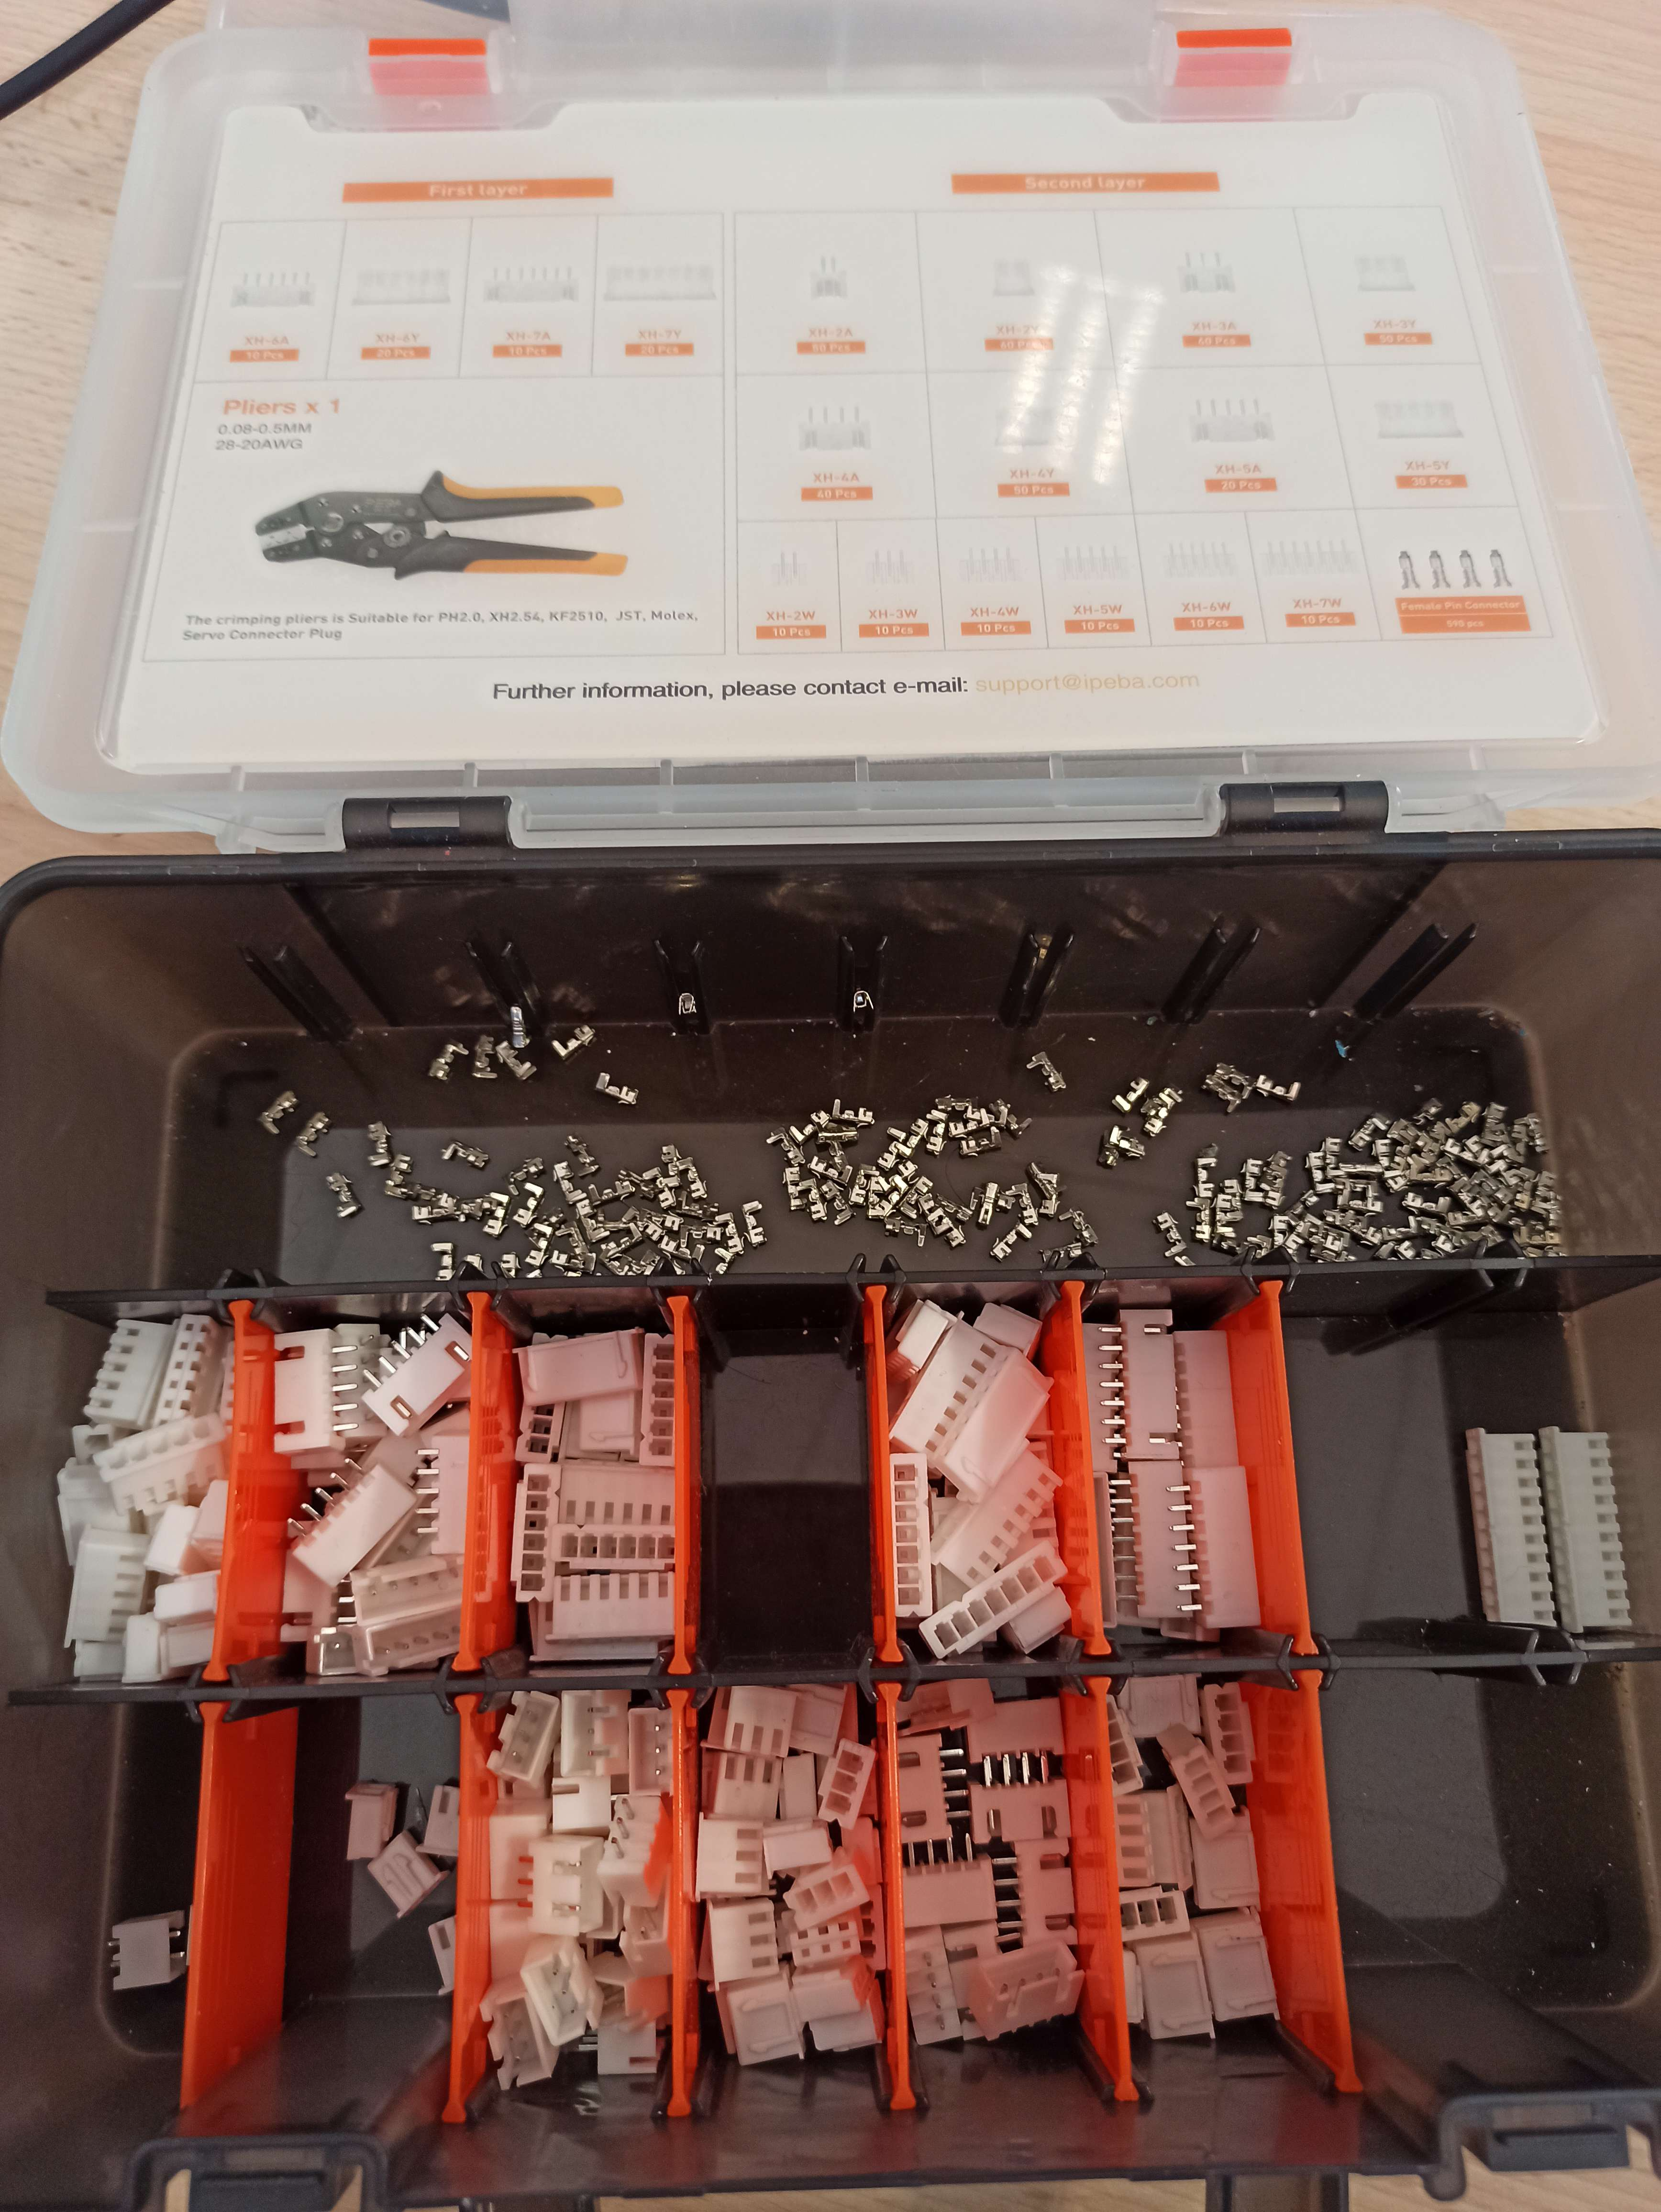
\includegraphics[width=0.28\textwidth]{images/boite_JST.jpg}
    \end{center}
    \captionsetup{labelformat=empty}
    \caption{La boîte à JST du local}
\end{figure}

\begin{figure}
    \begin{center}
        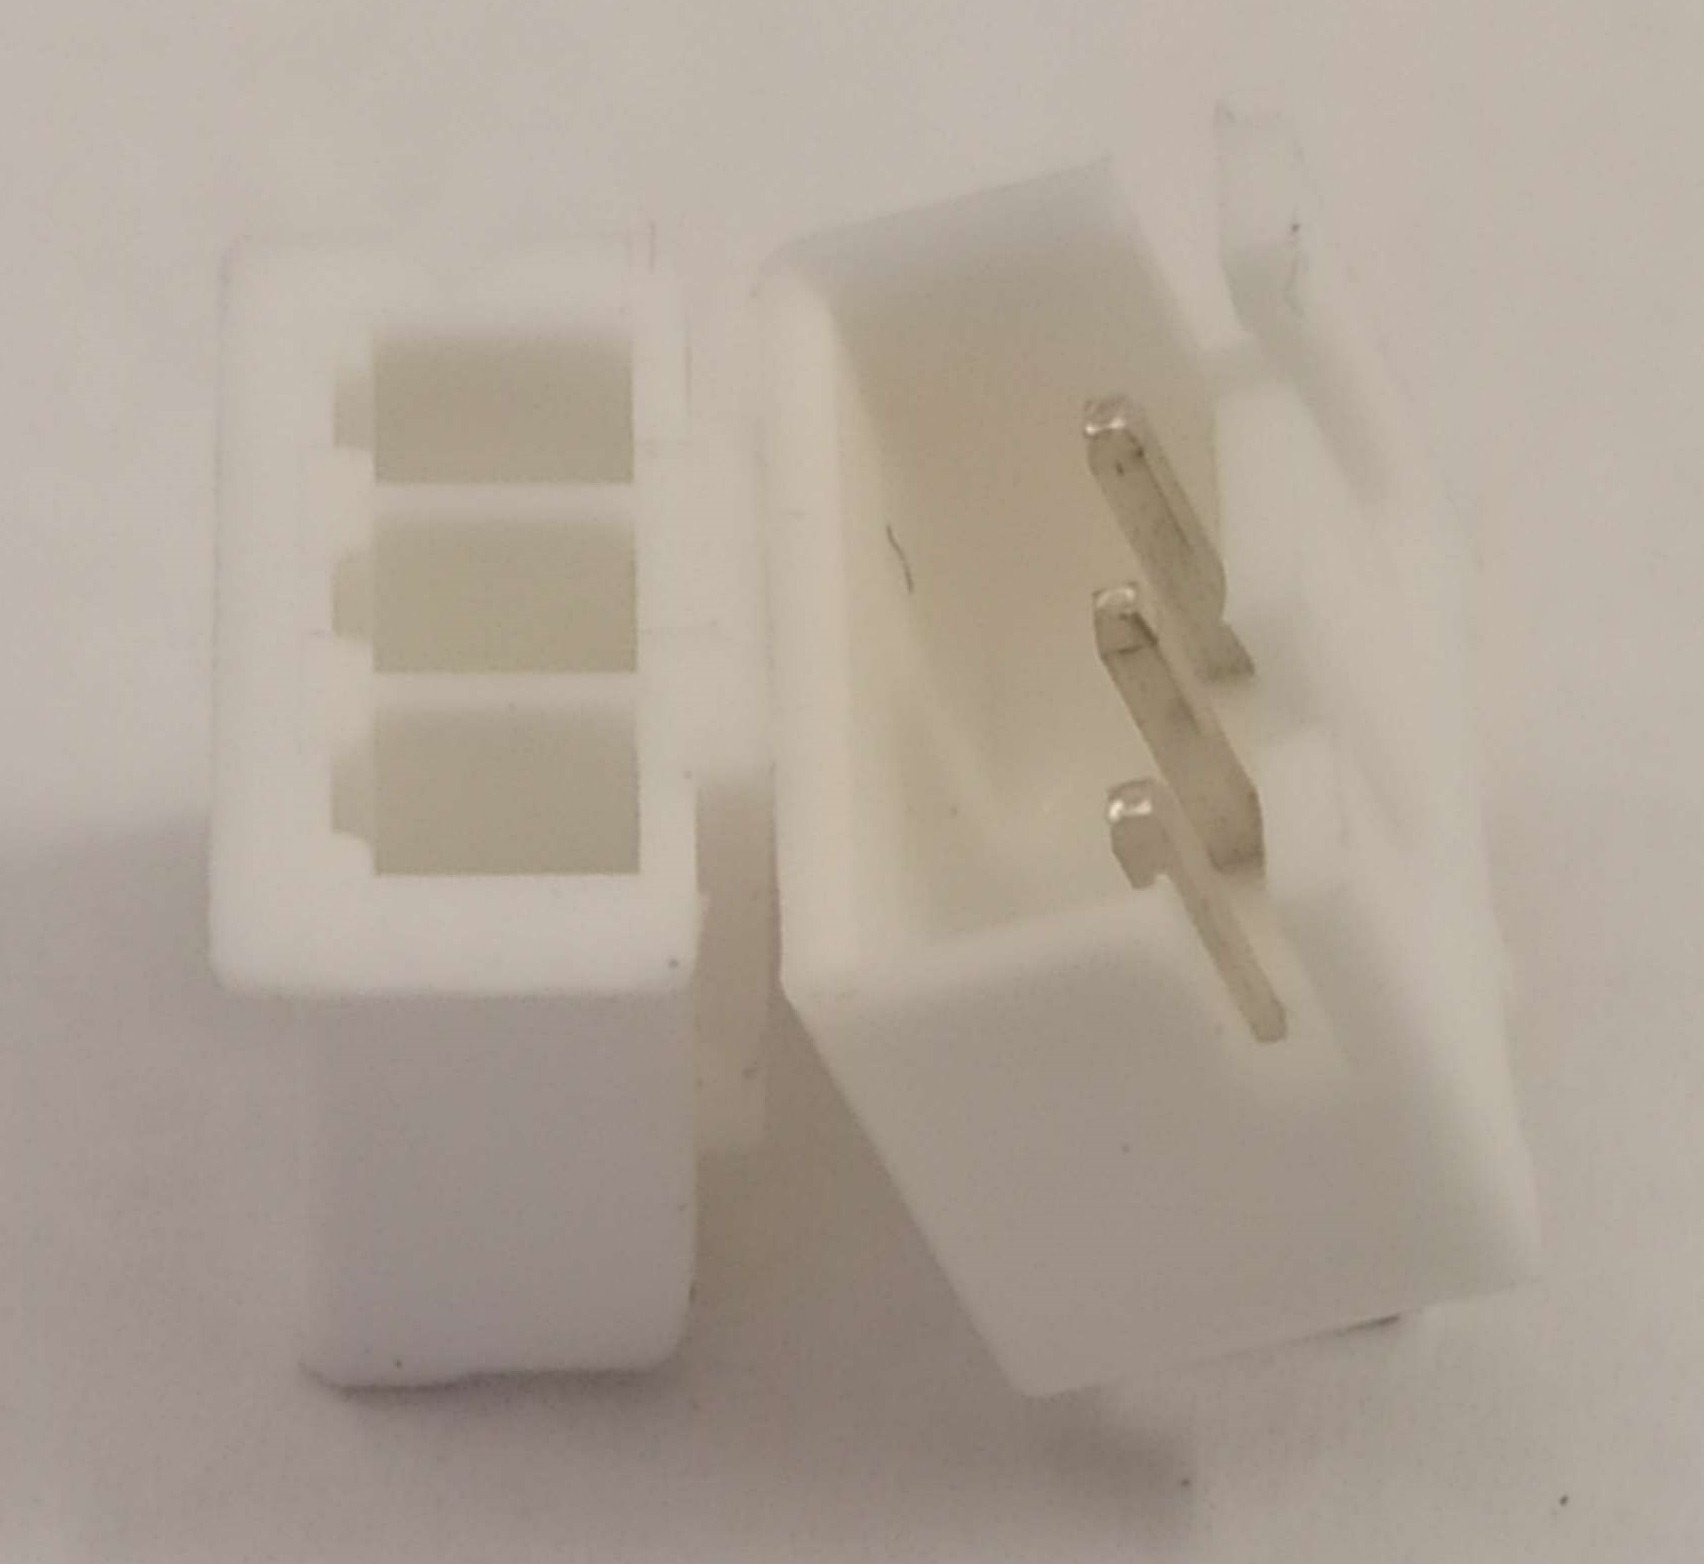
\includegraphics[width=0.28\textwidth]{images/JST_male_et_femelle.jpg}
    \end{center}
    \captionsetup{labelformat=empty}
    \caption{JST femelle à droite et JST mâle à gauche}
\end{figure}

\newpage
\section*{Étape 1: le dénudage}

\hspace{0.5cm} Après avoir choisit un câble de bon diamètre, de préférence souple et de bonne couleur, il faut le dénuder. 

\begin{minipage}{\textwidth}
    \vspace{0.5cm}
    \begin{center}
    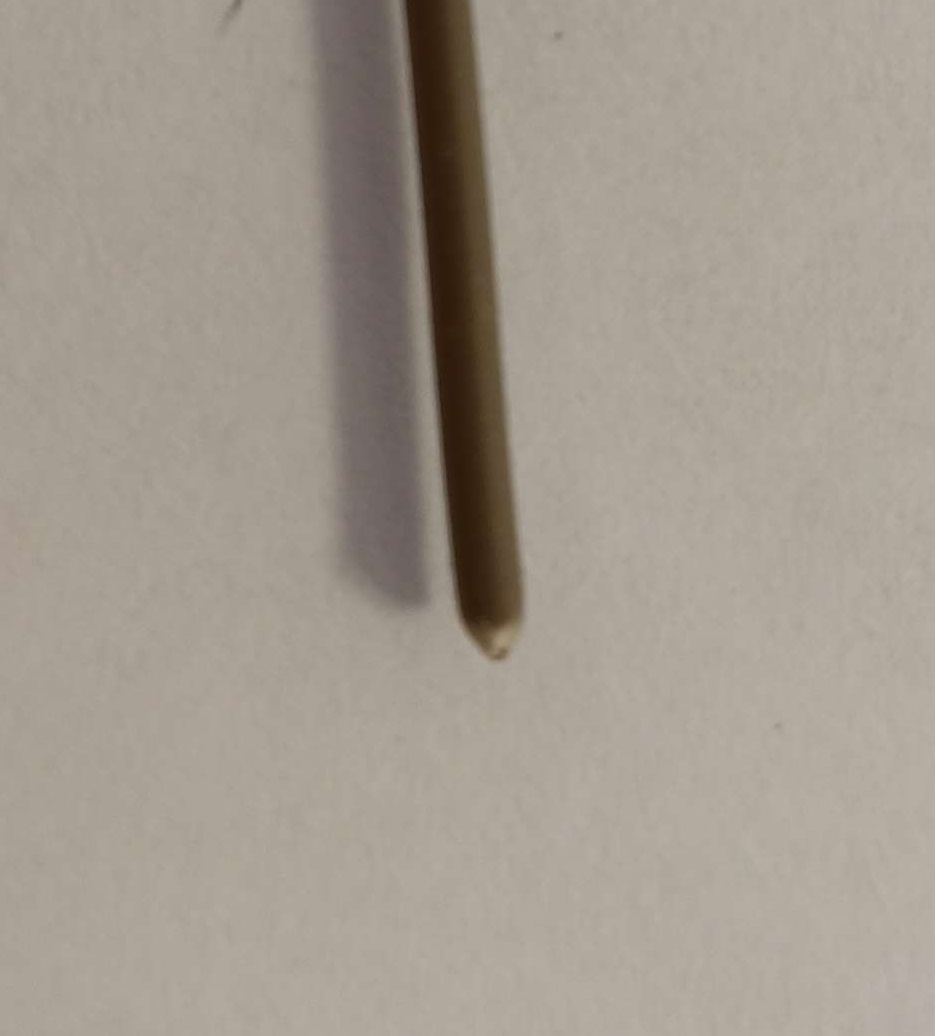
\includegraphics[width=0.28\textwidth]{images/fil_non_denude.jpg}
    \captionsetup{labelformat=empty}
    \captionof{figure}{Fil non dénudé}
    \end{center}
    \vspace{0.5cm}
\end{minipage}

D'abord, il faut définir la distance à dénuder. Inutile de dénuder le câble sur une longueur trop importante.

\begin{minipage}{\textwidth}
    \vspace{0.5cm}
    \begin{center}
    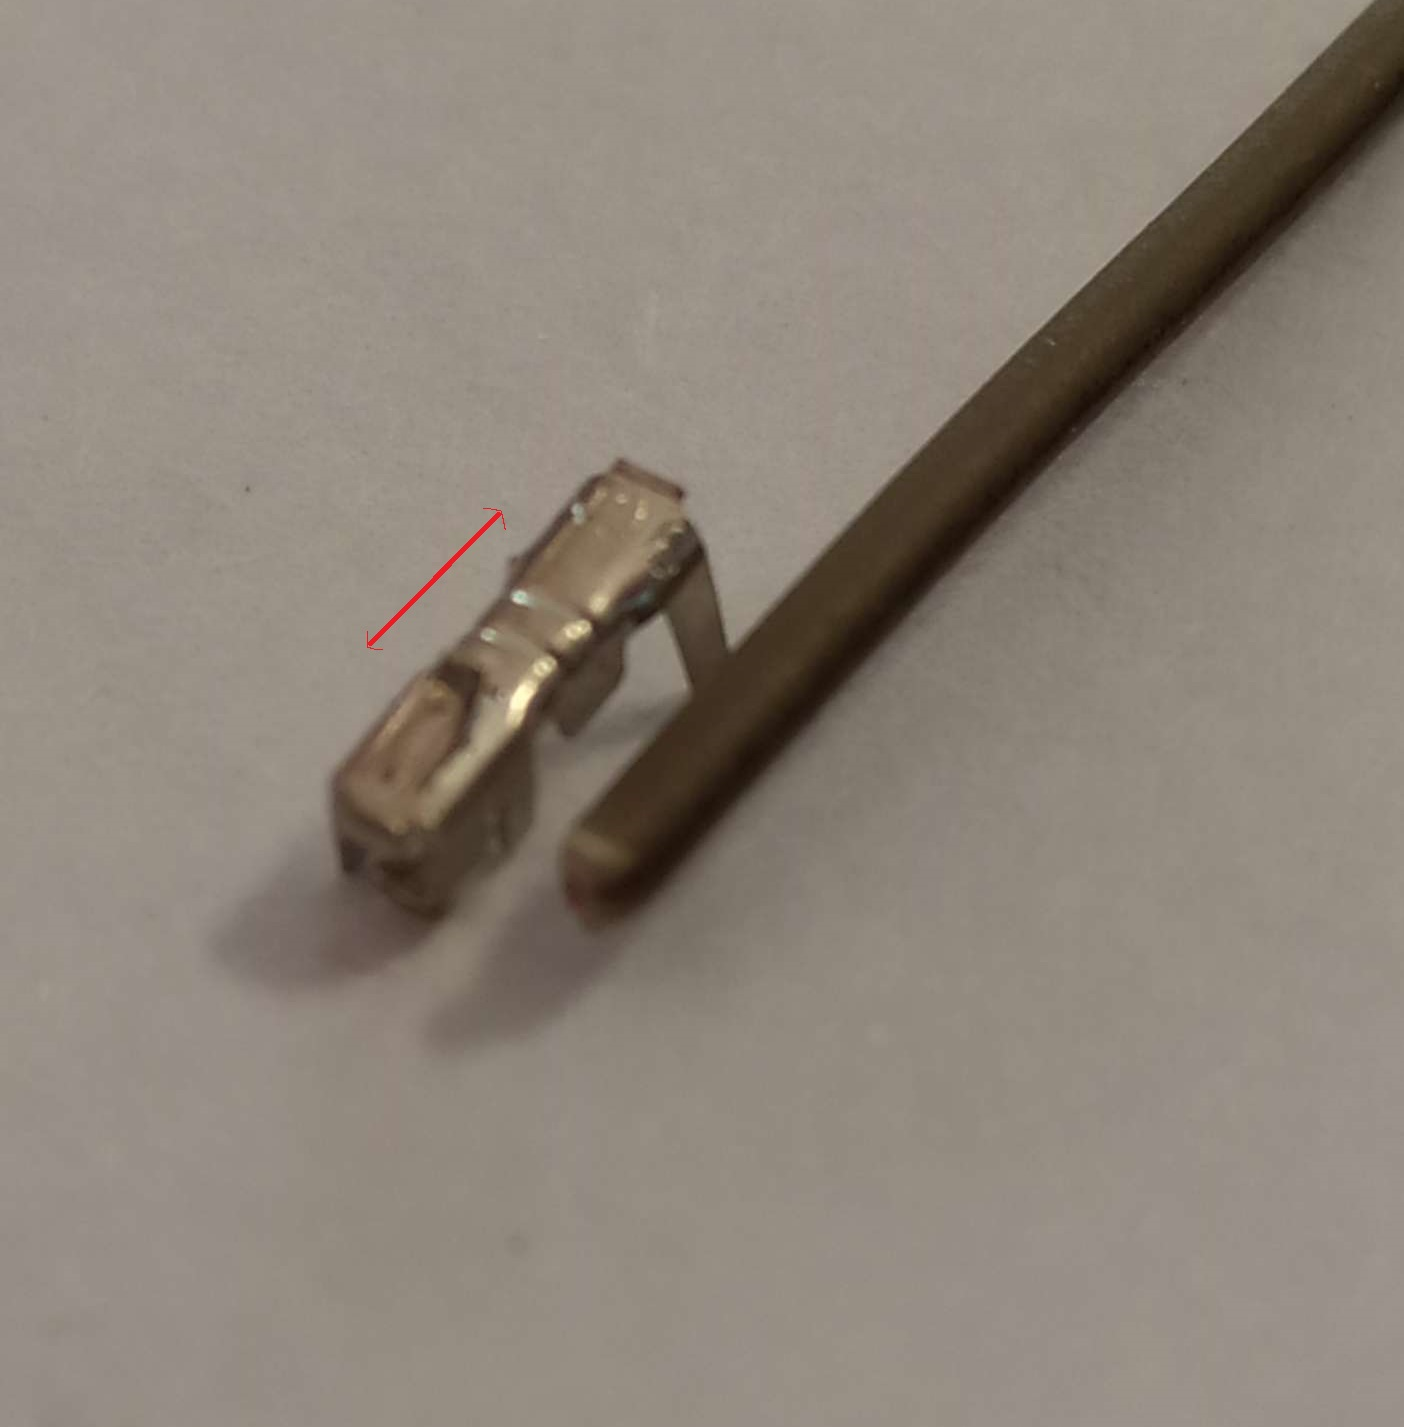
\includegraphics[width=0.4\textwidth]{images/choisir_longeur_a_denuder.jpg}
    \captionsetup{labelformat=empty}
    \captionof{figure}{La bonne longueur est représentée sur le trait rouge}
    \end{center}
    \vspace{0.5cm}
\end{minipage}

Pour trouver la distance de fil à dénuder, placez votre fil au-dessus de votre cosse (ici il s'agit d'un \textbf{XH 2.54 mm pitch female pin connectors}). 

\begin{minipage}{\textwidth}
    \vspace{0.5cm}
    \begin{center}
    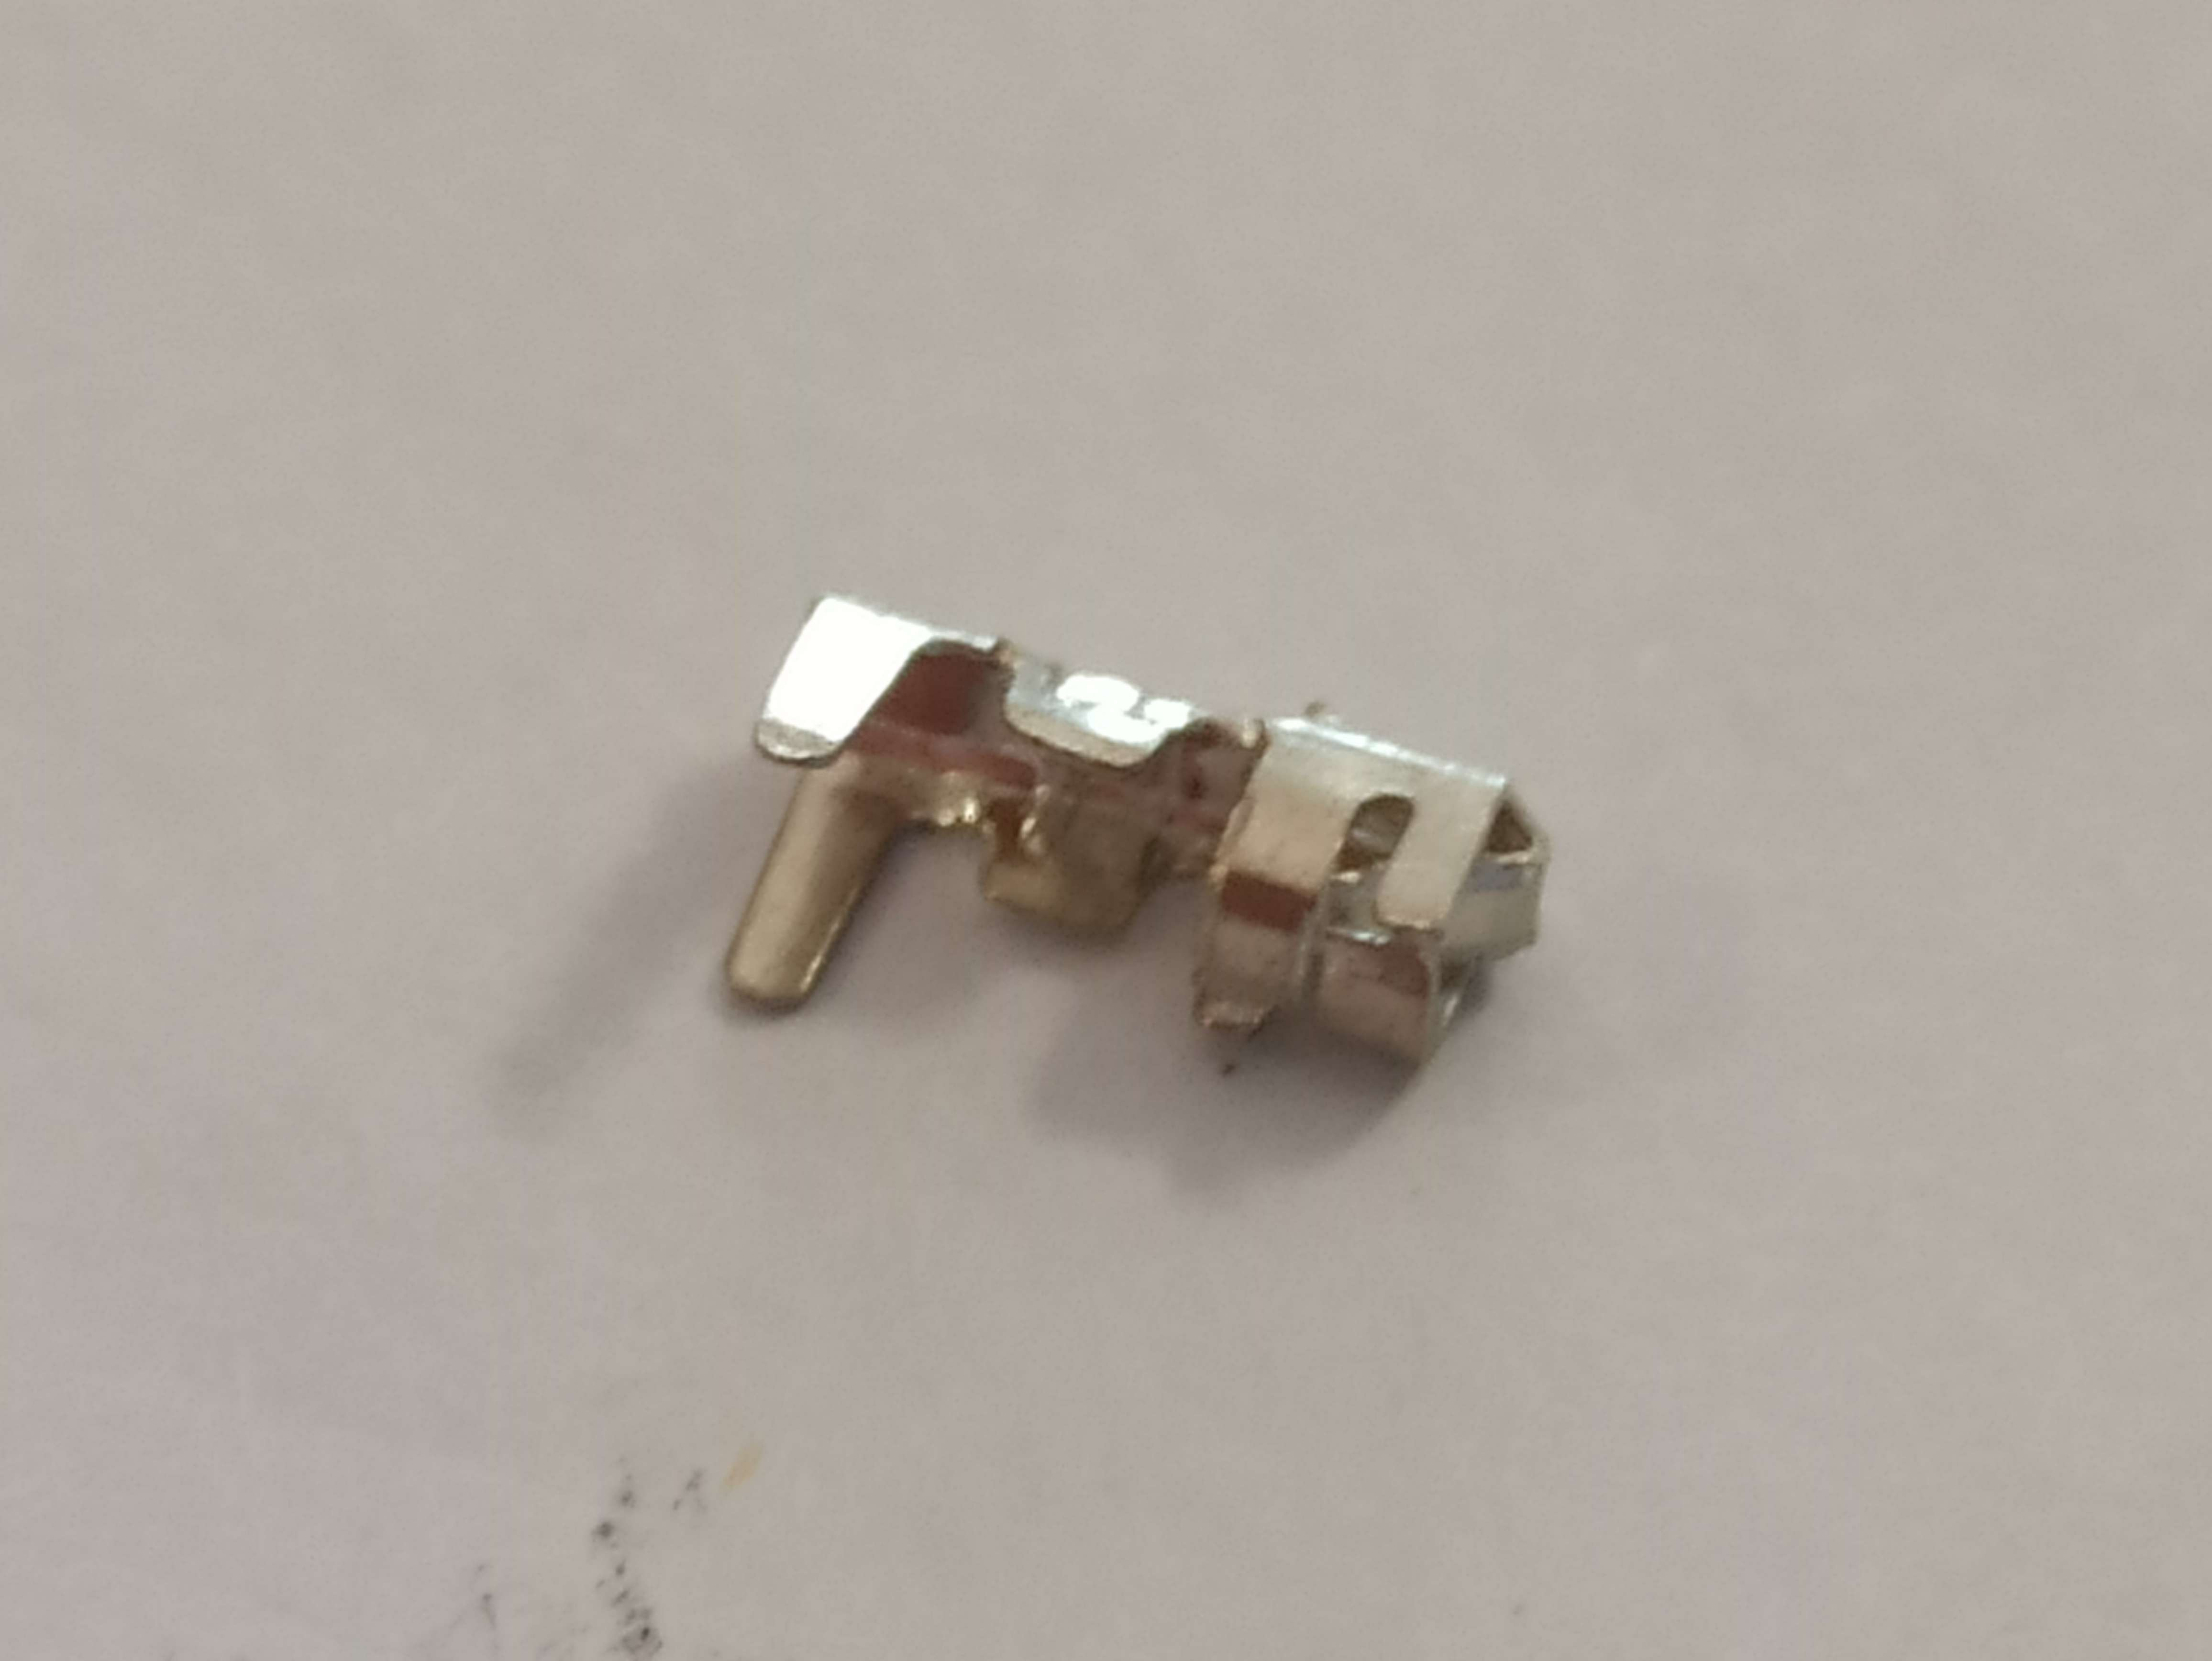
\includegraphics[width=0.28\textwidth]{images/cosse_JST.jpg}
    \captionsetup{labelformat=empty}
    \captionof{figure}{Une cosse JST XH}
    \end{center}
    \vspace{0.5cm}
\end{minipage}

Regardez les deux images ci-dessous, la première c'est ce que l'on a, la deuxième ce que l'on veut. Remarquez que les languettes de métal vont se replier pour serrer le plastique du câble et que juste après on a le fil dénuder. Également, notez que les filaments ne dépassent pas de la cosse.

\begin{figure}[h]
    \begin{minipage}{0.45\textwidth}
        \centering
        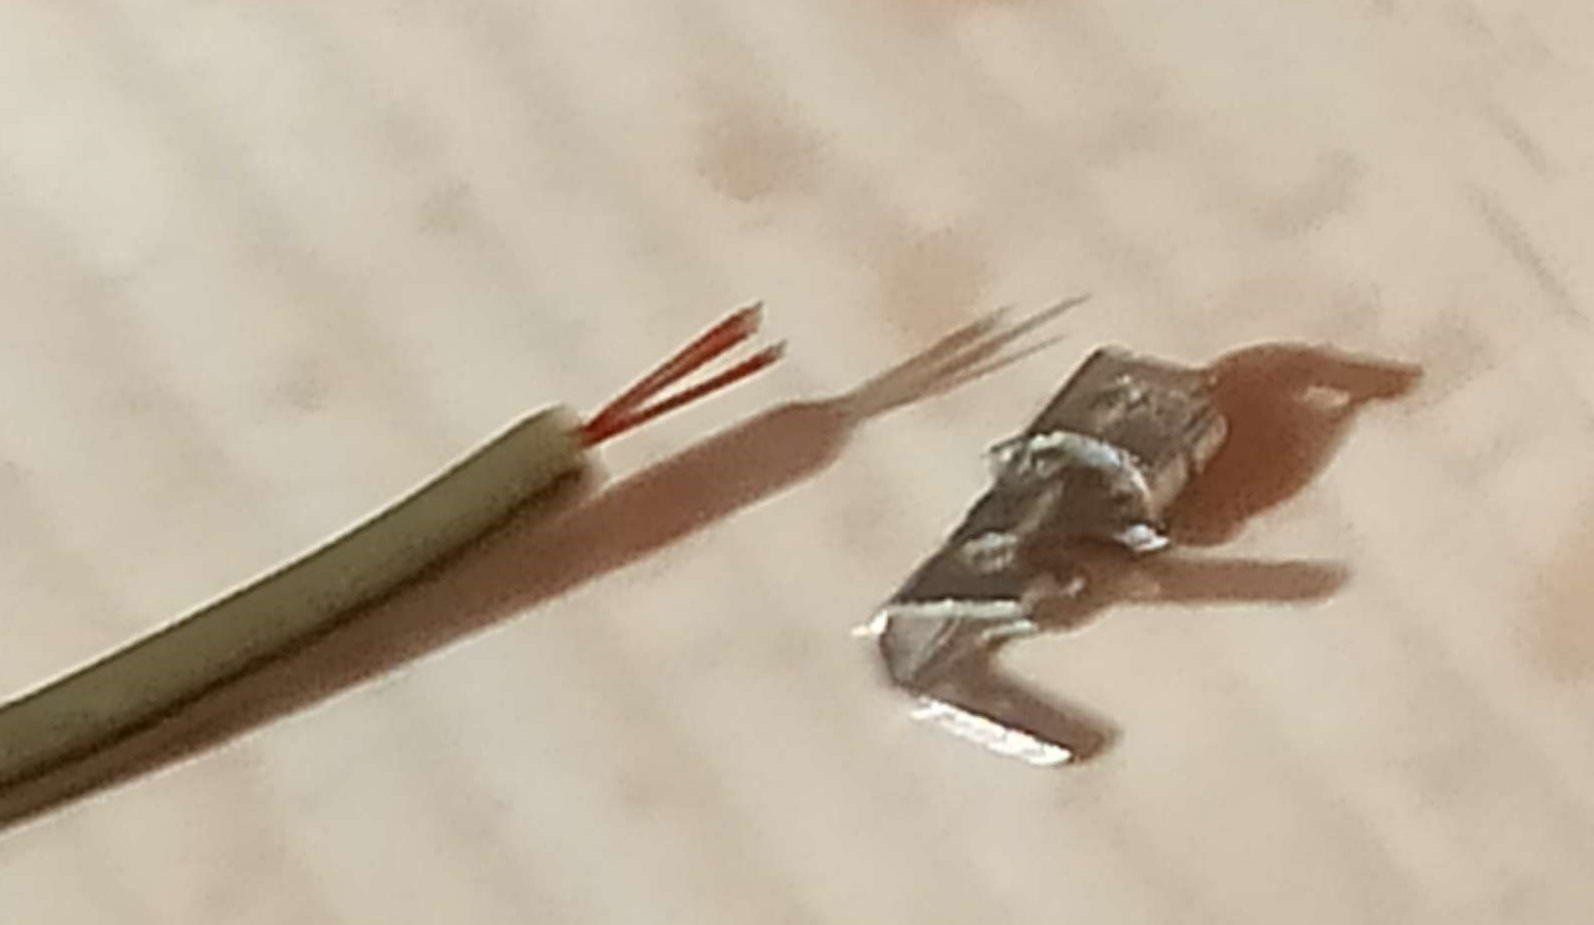
\includegraphics[width=\linewidth]{images/apres_denudage.jpg}
        \captionsetup{labelformat=empty}
        \caption{}
        \label{fig:image1}
    \end{minipage}
    \hfill
    \begin{minipage}{0.45\textwidth}
        \centering
        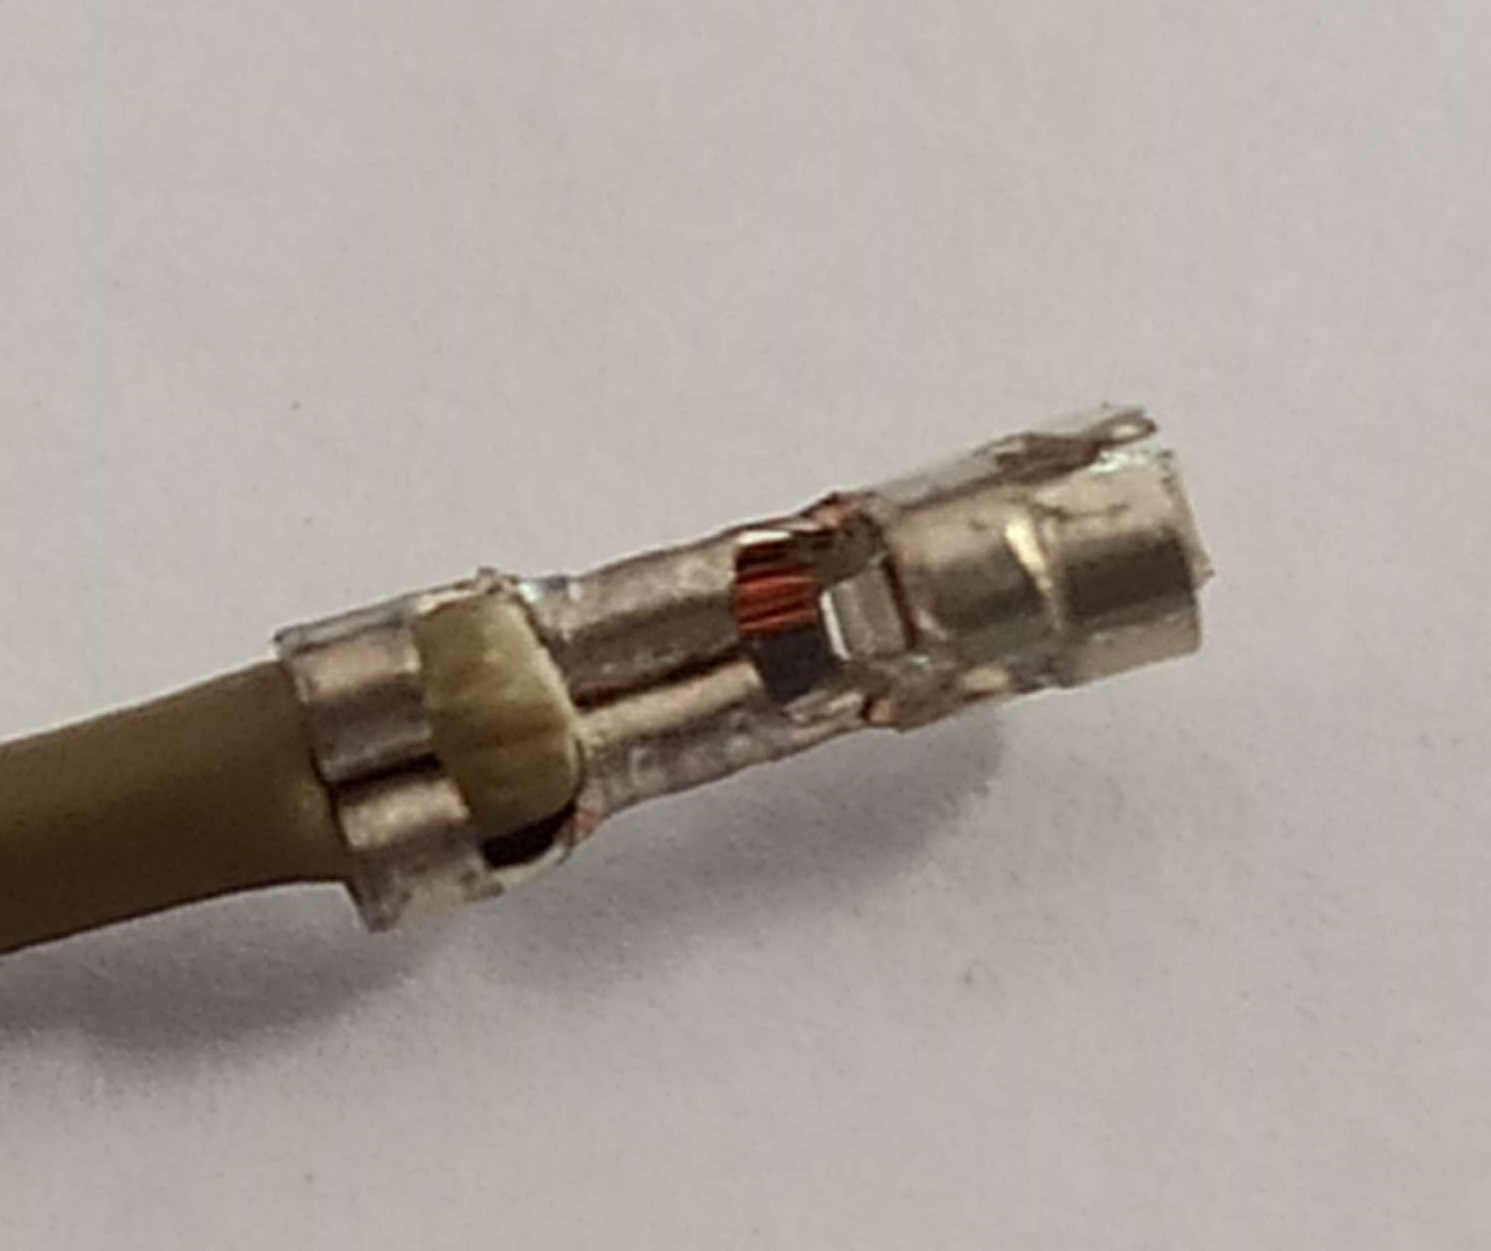
\includegraphics[width=\linewidth]{images/sertissage_finit.jpg}
        \captionsetup{labelformat=empty}
        \caption{}
        \label{fig:image2}
    \end{minipage}
\end{figure}

Pour le dénudage, on utilise une pince à dénuder. Par exemple, au local, on a la pince à dénuder rouge. Choissisez le bon diamètre pour dénuder: en cas de doute, commencez par un diamètre plus gros, et diminuer de diamètre jusqu'à ce que le câble soit correctement dénudé.

\begin{figure}[h]
    \begin{minipage}{0.45\textwidth}
        \centering
        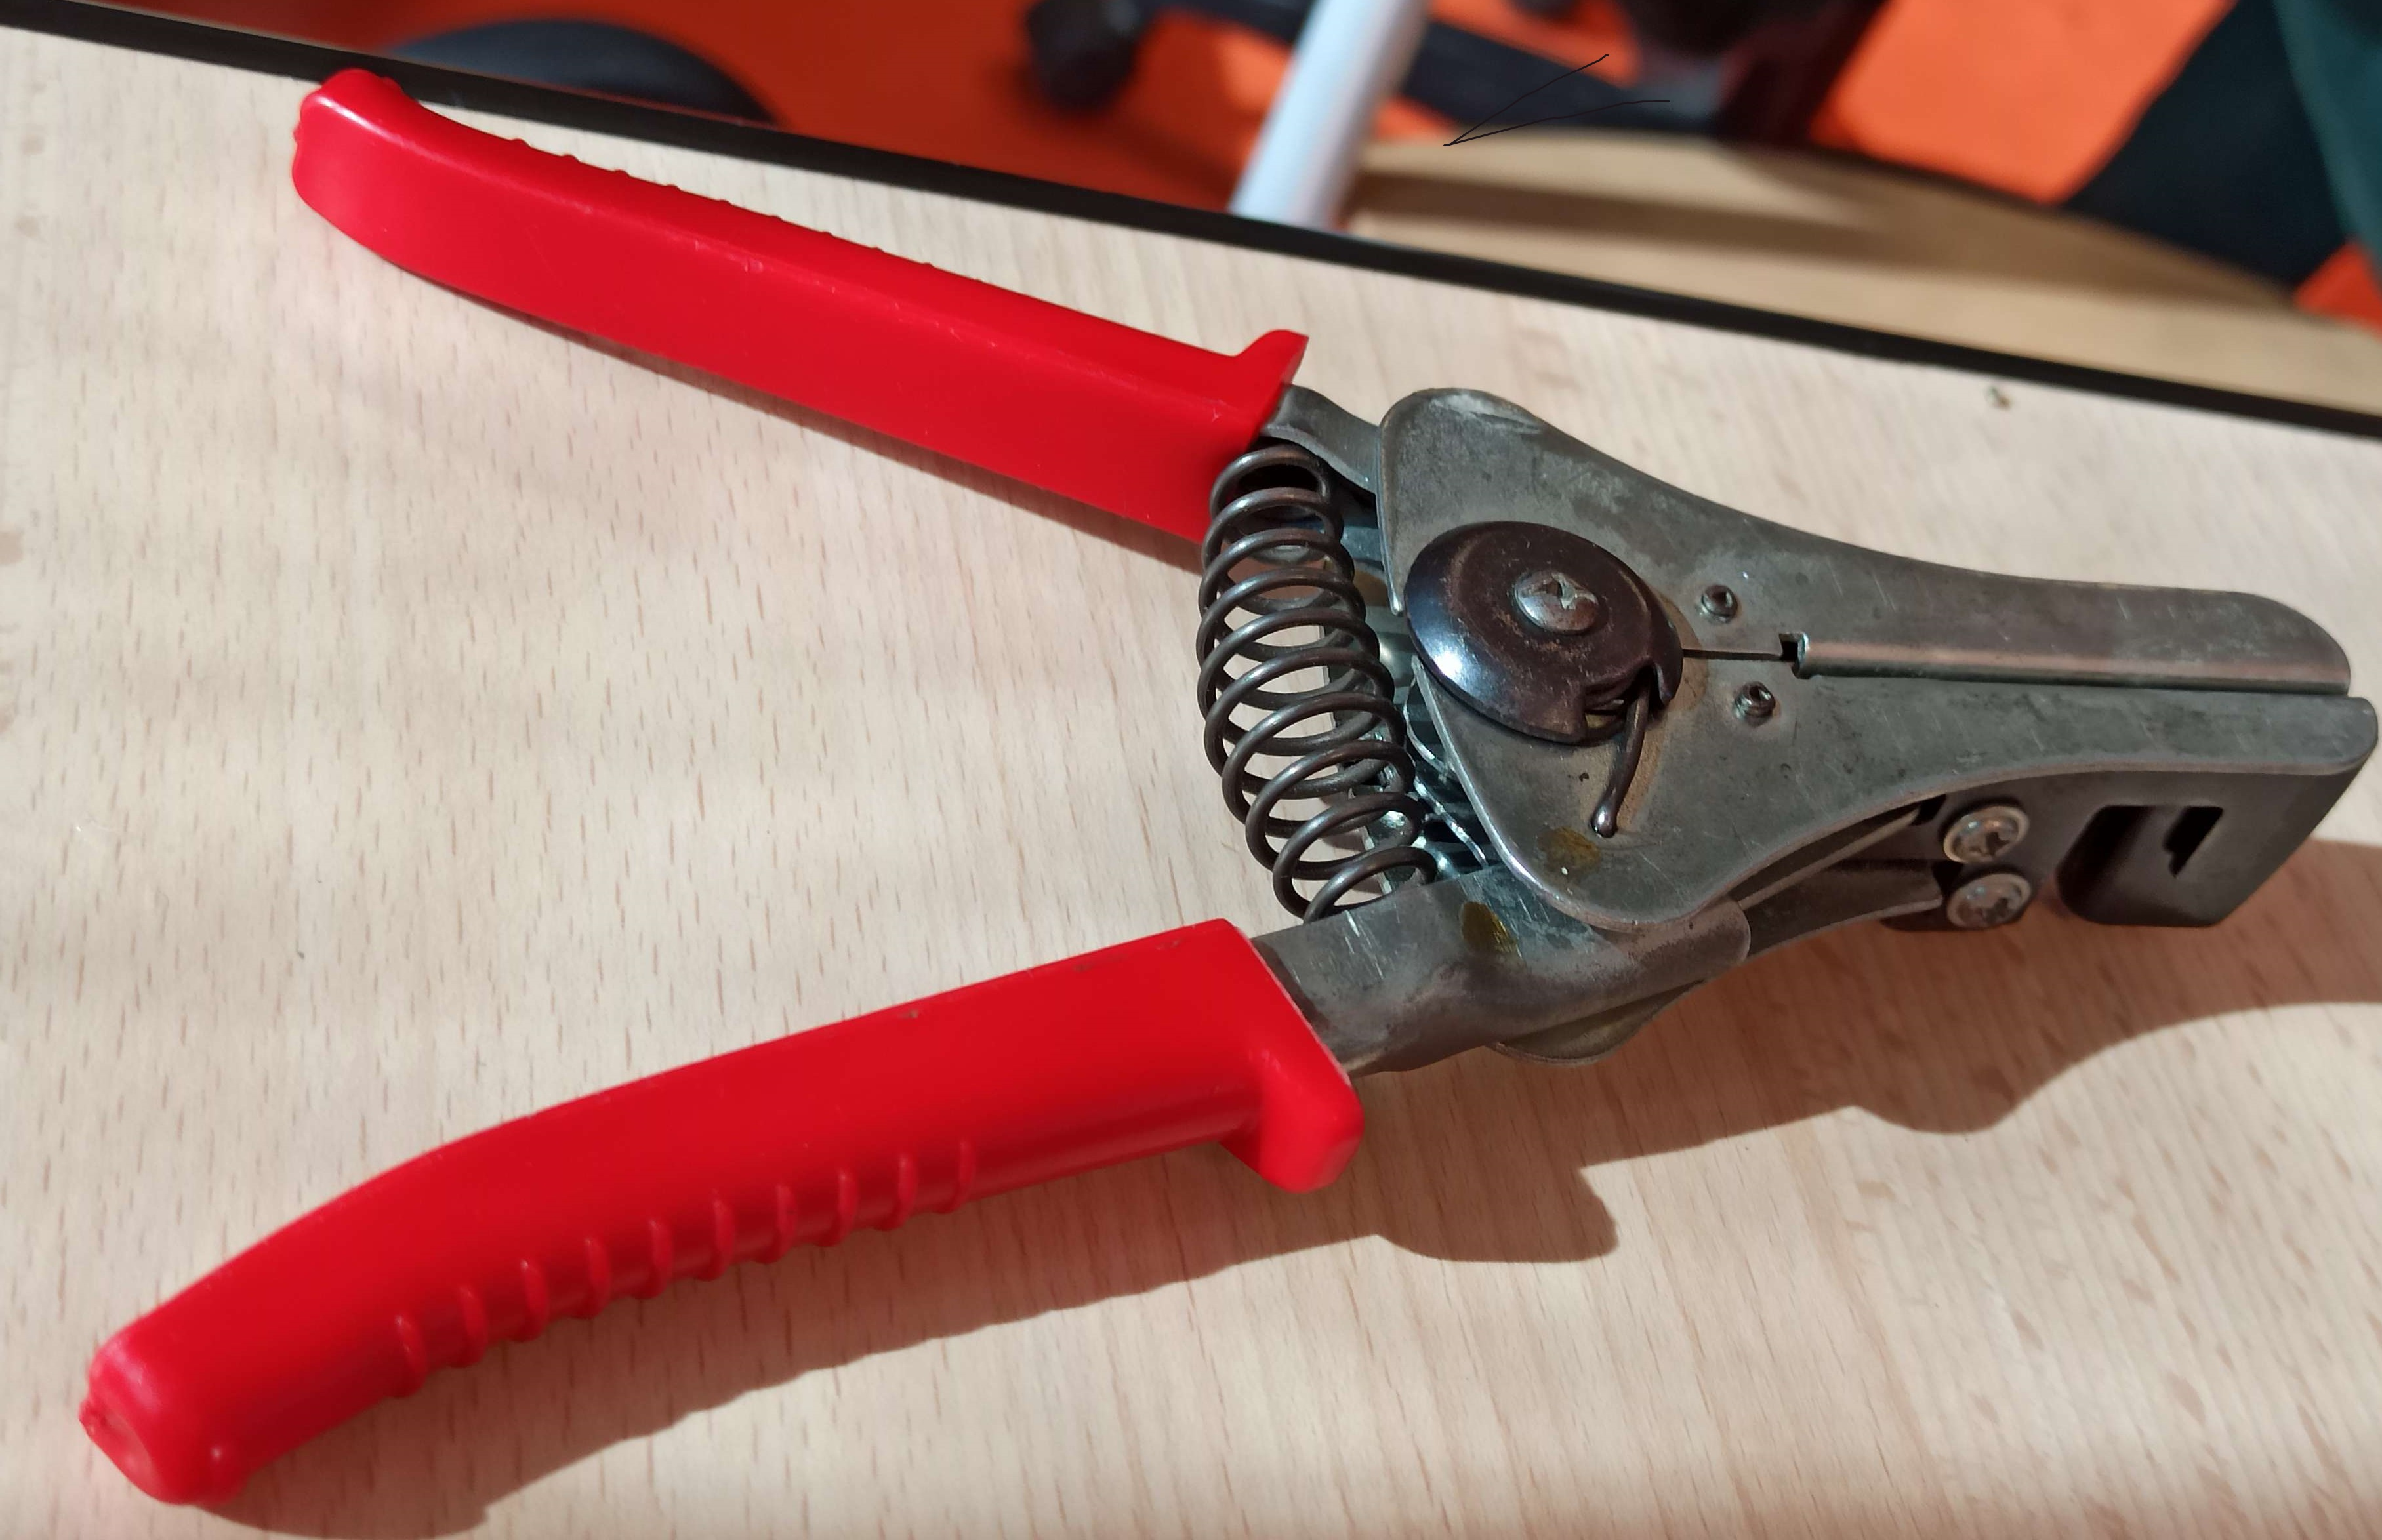
\includegraphics[width=\linewidth]{images/pince_pour_denuder.jpg}
        \captionsetup{labelformat=empty}
        \caption{Pince à dénuder}
        \label{fig:image1}
    \end{minipage}
    \hfill
    \begin{minipage}{0.45\textwidth}
        \centering
        \includegraphics[width=\linewidth]{images/fil_dans_pince_a_denuder.jpg}
        \captionsetup{labelformat=empty}
        \caption{}
        \label{fig:image2}
    \end{minipage}
\end{figure}

\newpage
\section*{Étape 2: le sertissage}

Maintenant, il faut utiliser une pince à sertir. On en a deux au local AREM, attention pour les JST il faut utiliser la pince jaune, c'est celle qui était livrée avec les connecteurs et qui est par conséquent adaptée. 

\begin{minipage}{\textwidth}
    \vspace{0.5cm}
    \begin{center}
    \rotatebox{90}{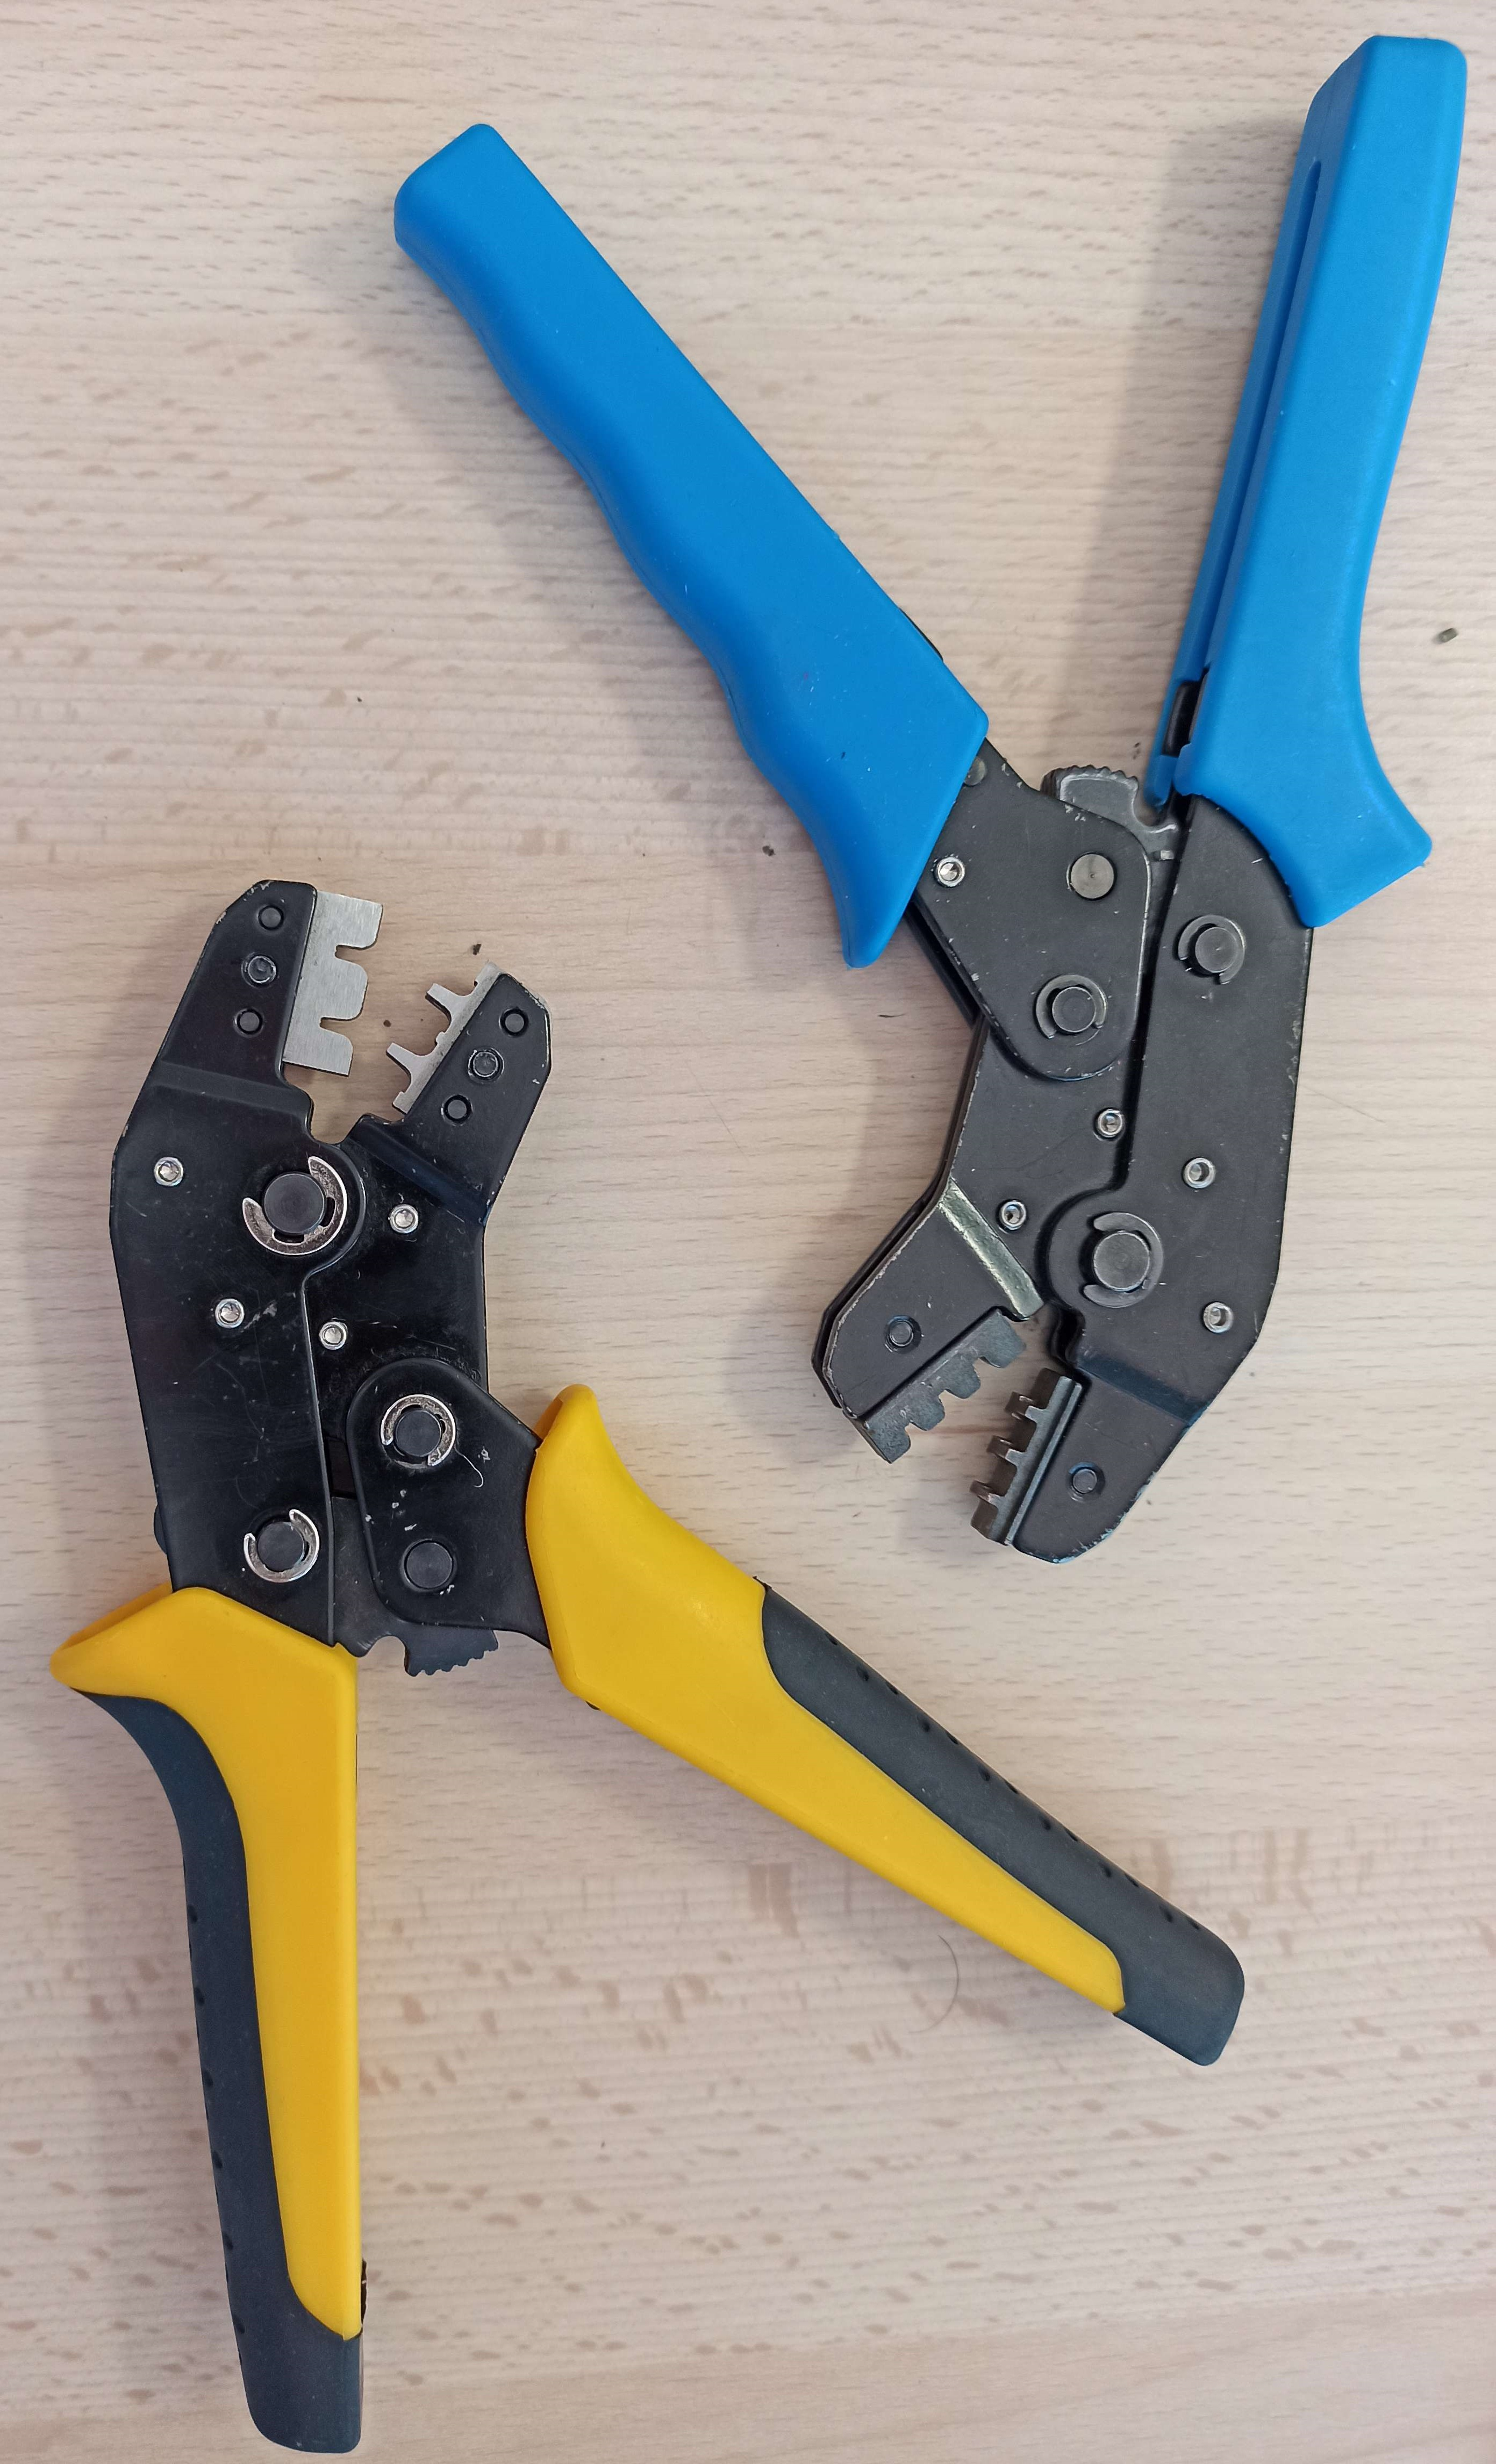
\includegraphics[width=0.4\textwidth]{images/pinces_pour_sertir.jpg}}
    \captionsetup{labelformat=empty}
    \captionof{figure}{}
    \end{center}
    \vspace{0.5cm}
\end{minipage}

Mettez la cosse dans l'emplacement adapté. Attention, notez qu'il y a également un sens. En d'autres mots, dans l'emplacement pour la cosse, il y a une partie plus profonde que l'autre, c'est là que l'on va mettre la partie de la cosse où il y a les languettes. Faîtes bien comme sur les photos.  

\begin{figure}[h]
    \begin{minipage}{0.45\textwidth}
        \centering
        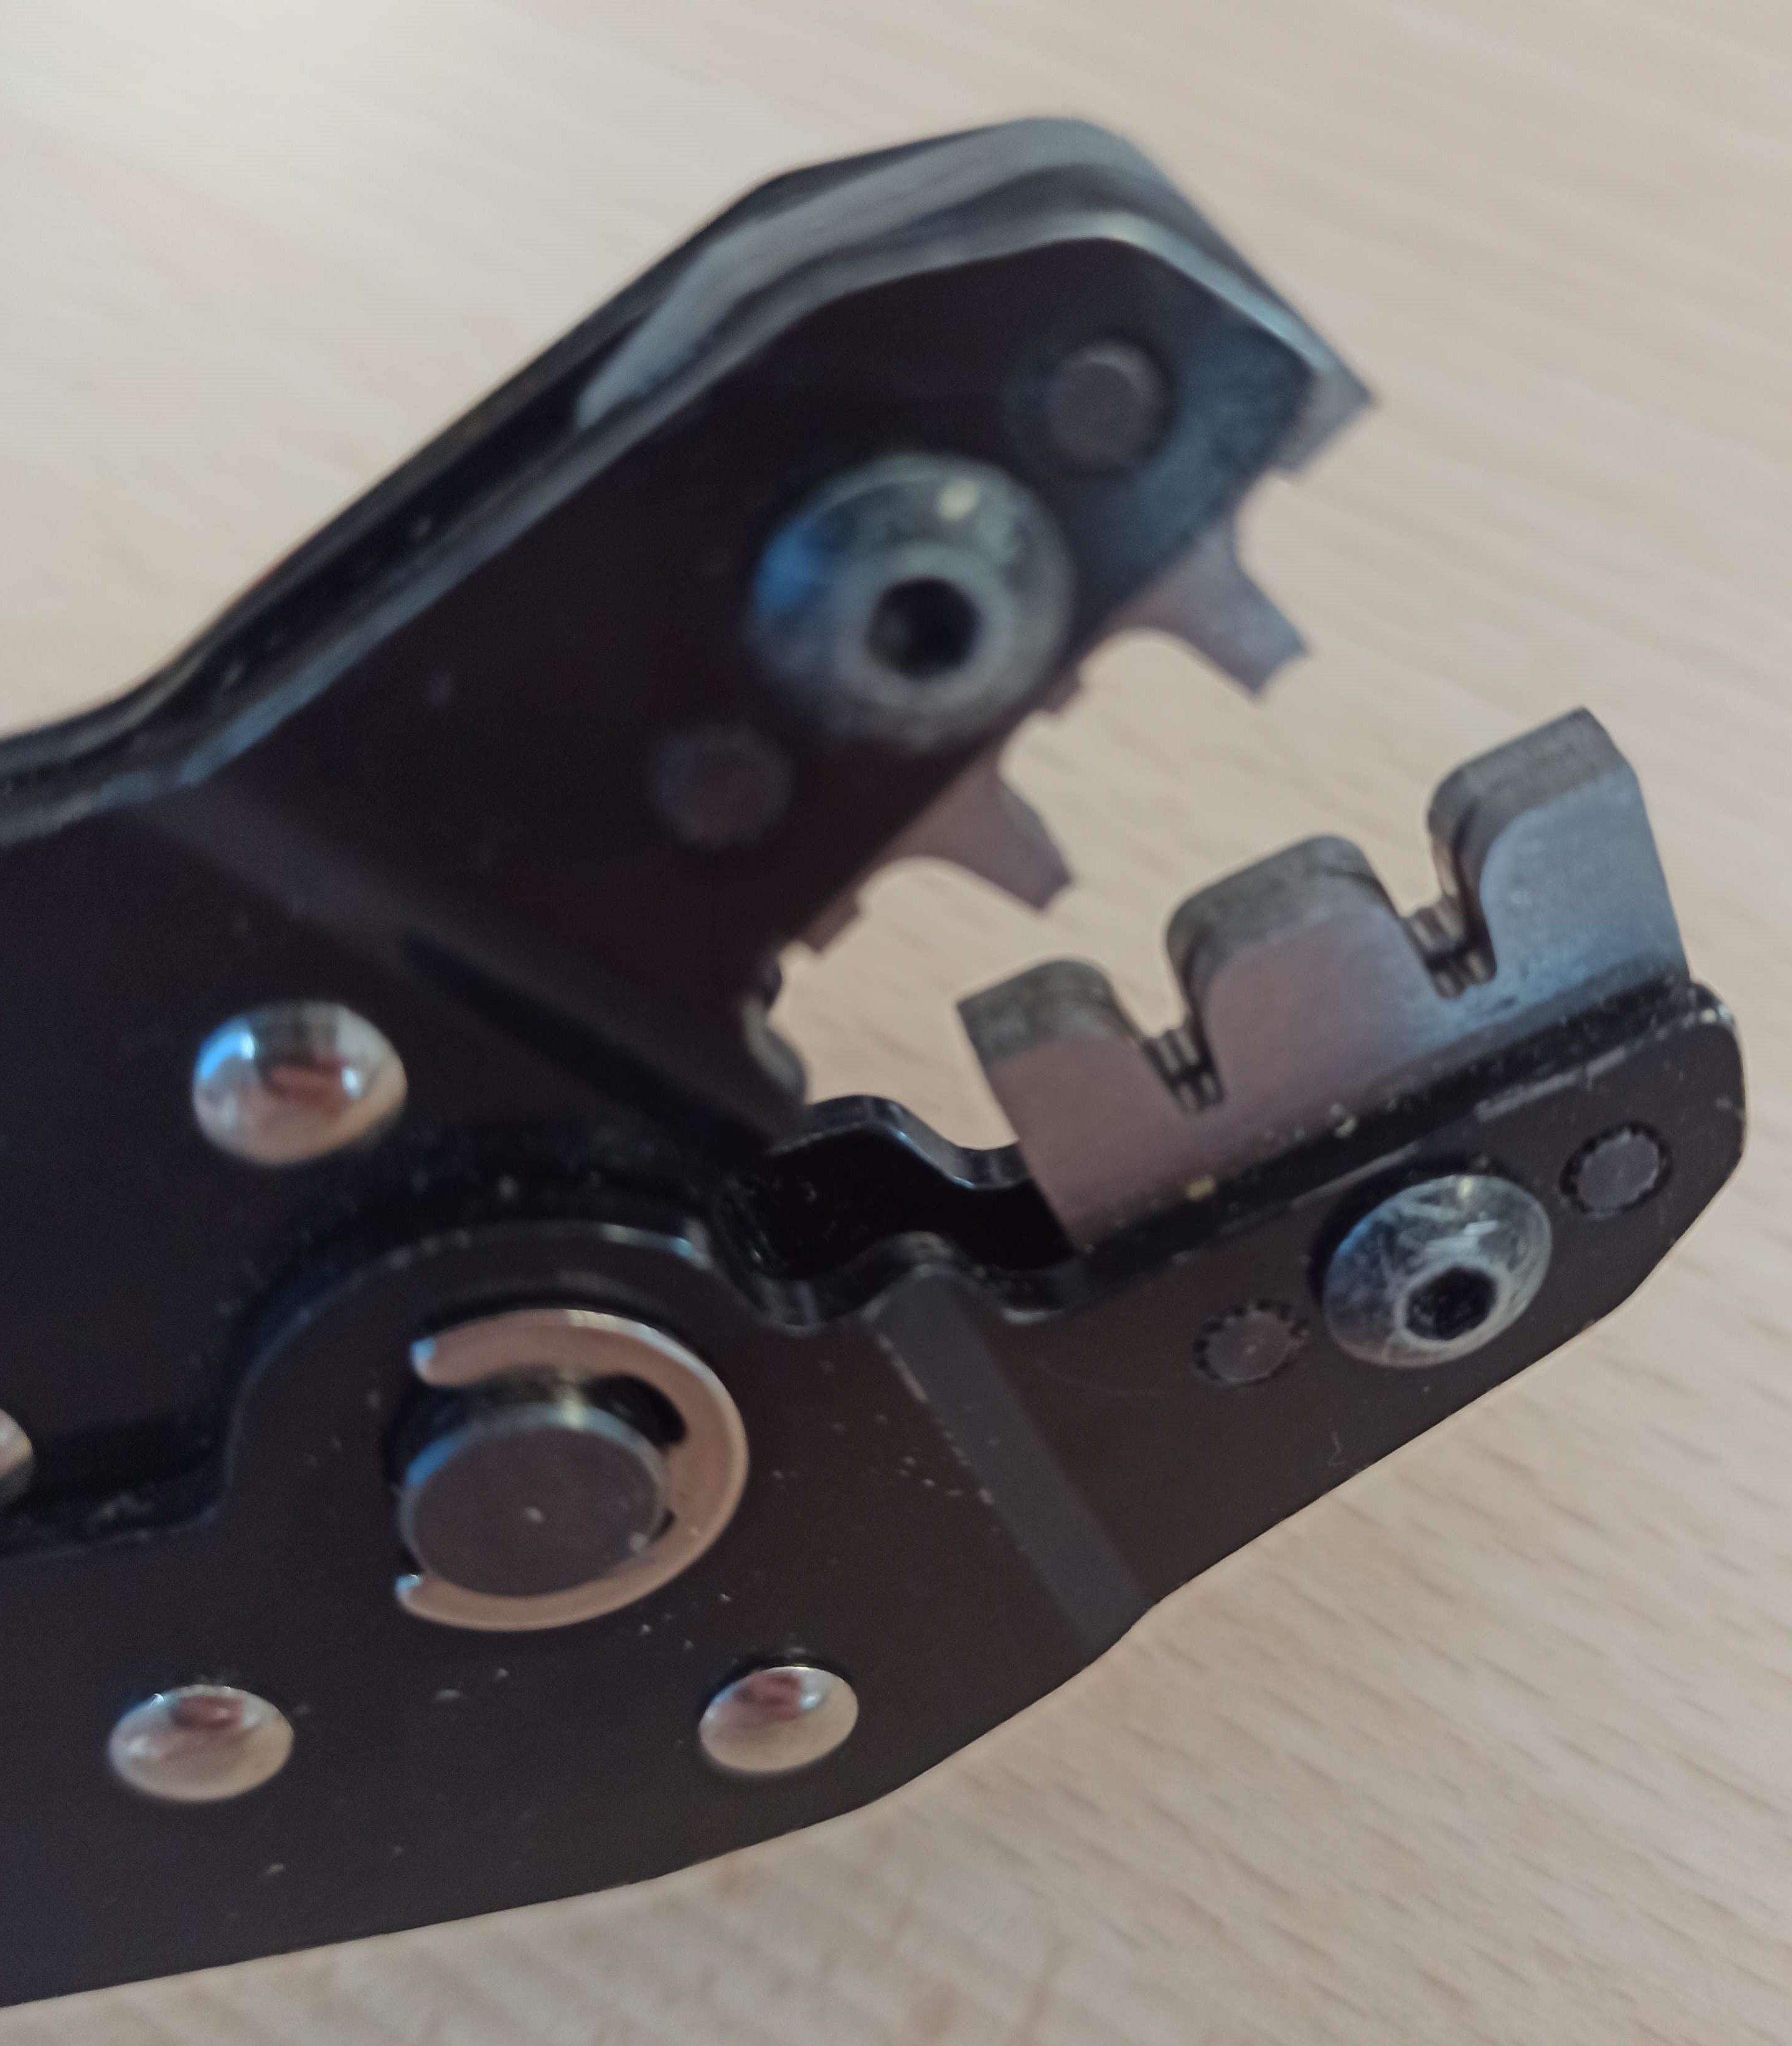
\includegraphics[width=\linewidth]{images/pince_sertir_emplacement_cosse_JST.jpg}
        \captionsetup{labelformat=empty}
        \caption{}
        \label{fig:image1}
    \end{minipage}
    \hfill
    \begin{minipage}{0.45\textwidth}
        \centering
        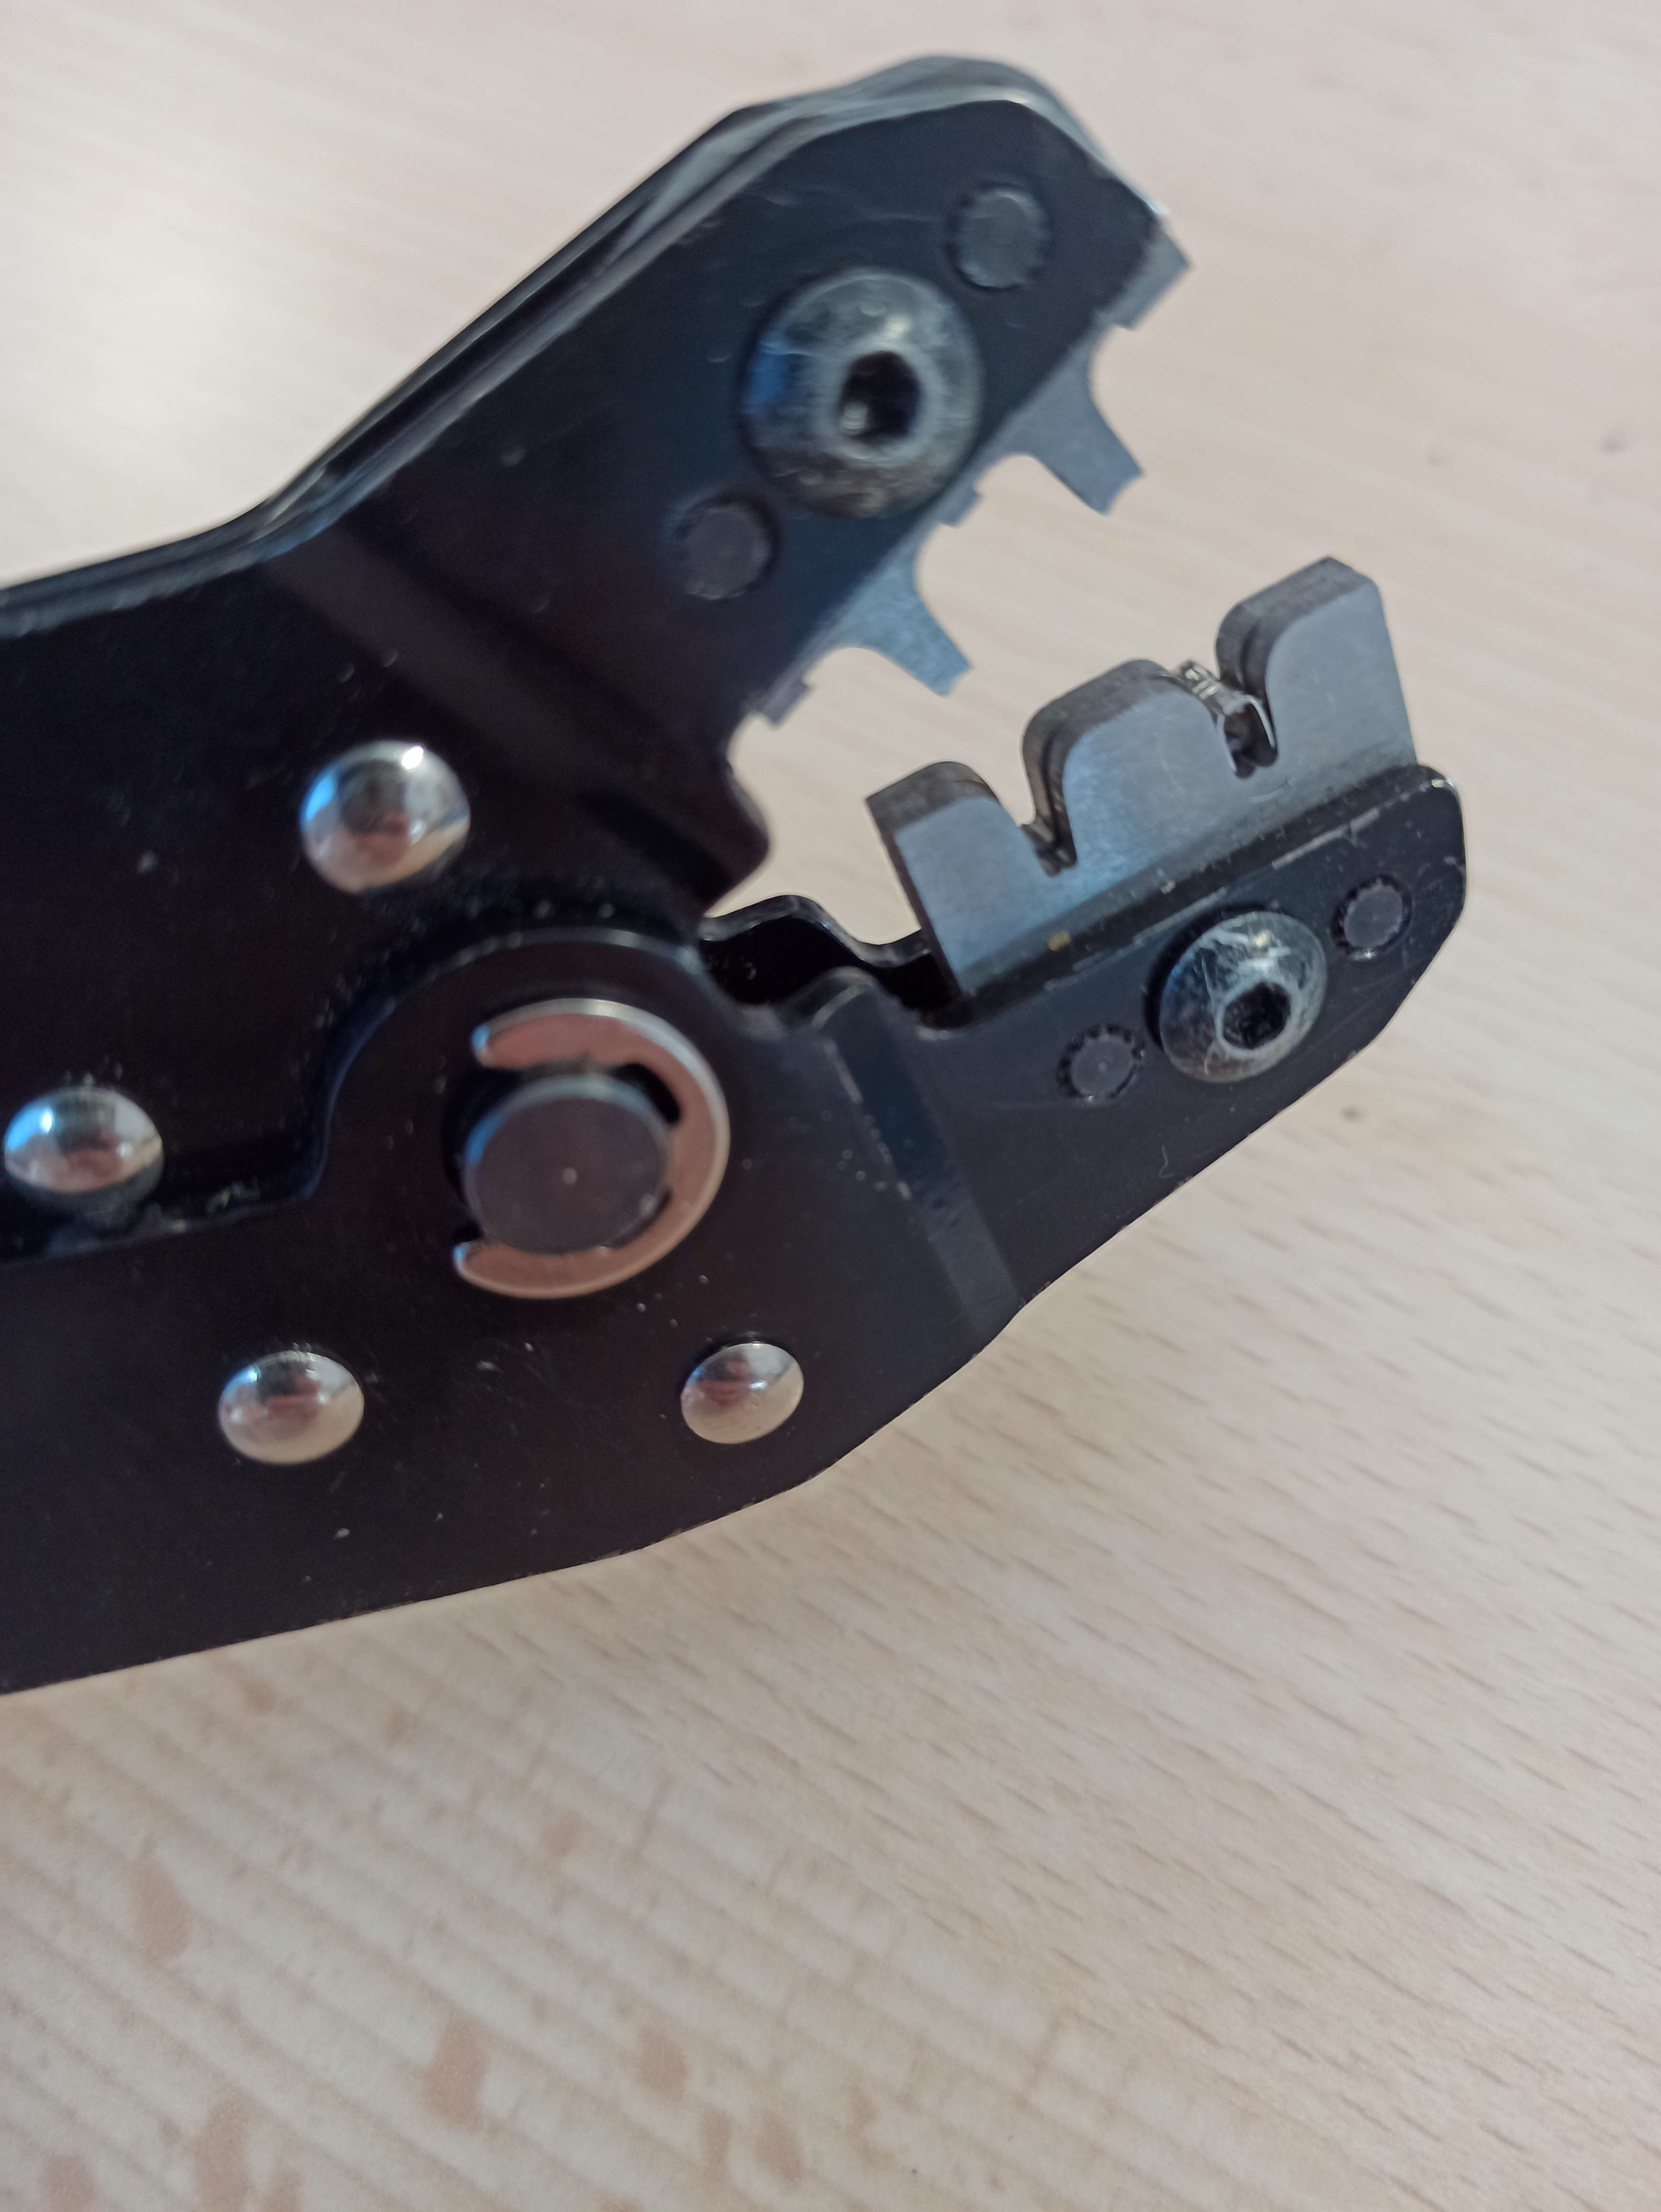
\includegraphics[width=\linewidth]{images/cosse_dans_pince_sertir.jpg}
        \captionsetup{labelformat=empty}
        \caption{}
        \label{fig:image2}
    \end{minipage}
\end{figure}

\newpage
Ensuite enfoncez la pince jusqu'au niveau de la cosse comme sur la photo:

\begin{minipage}{\textwidth}
    \vspace{0.5cm}
    \begin{center}
    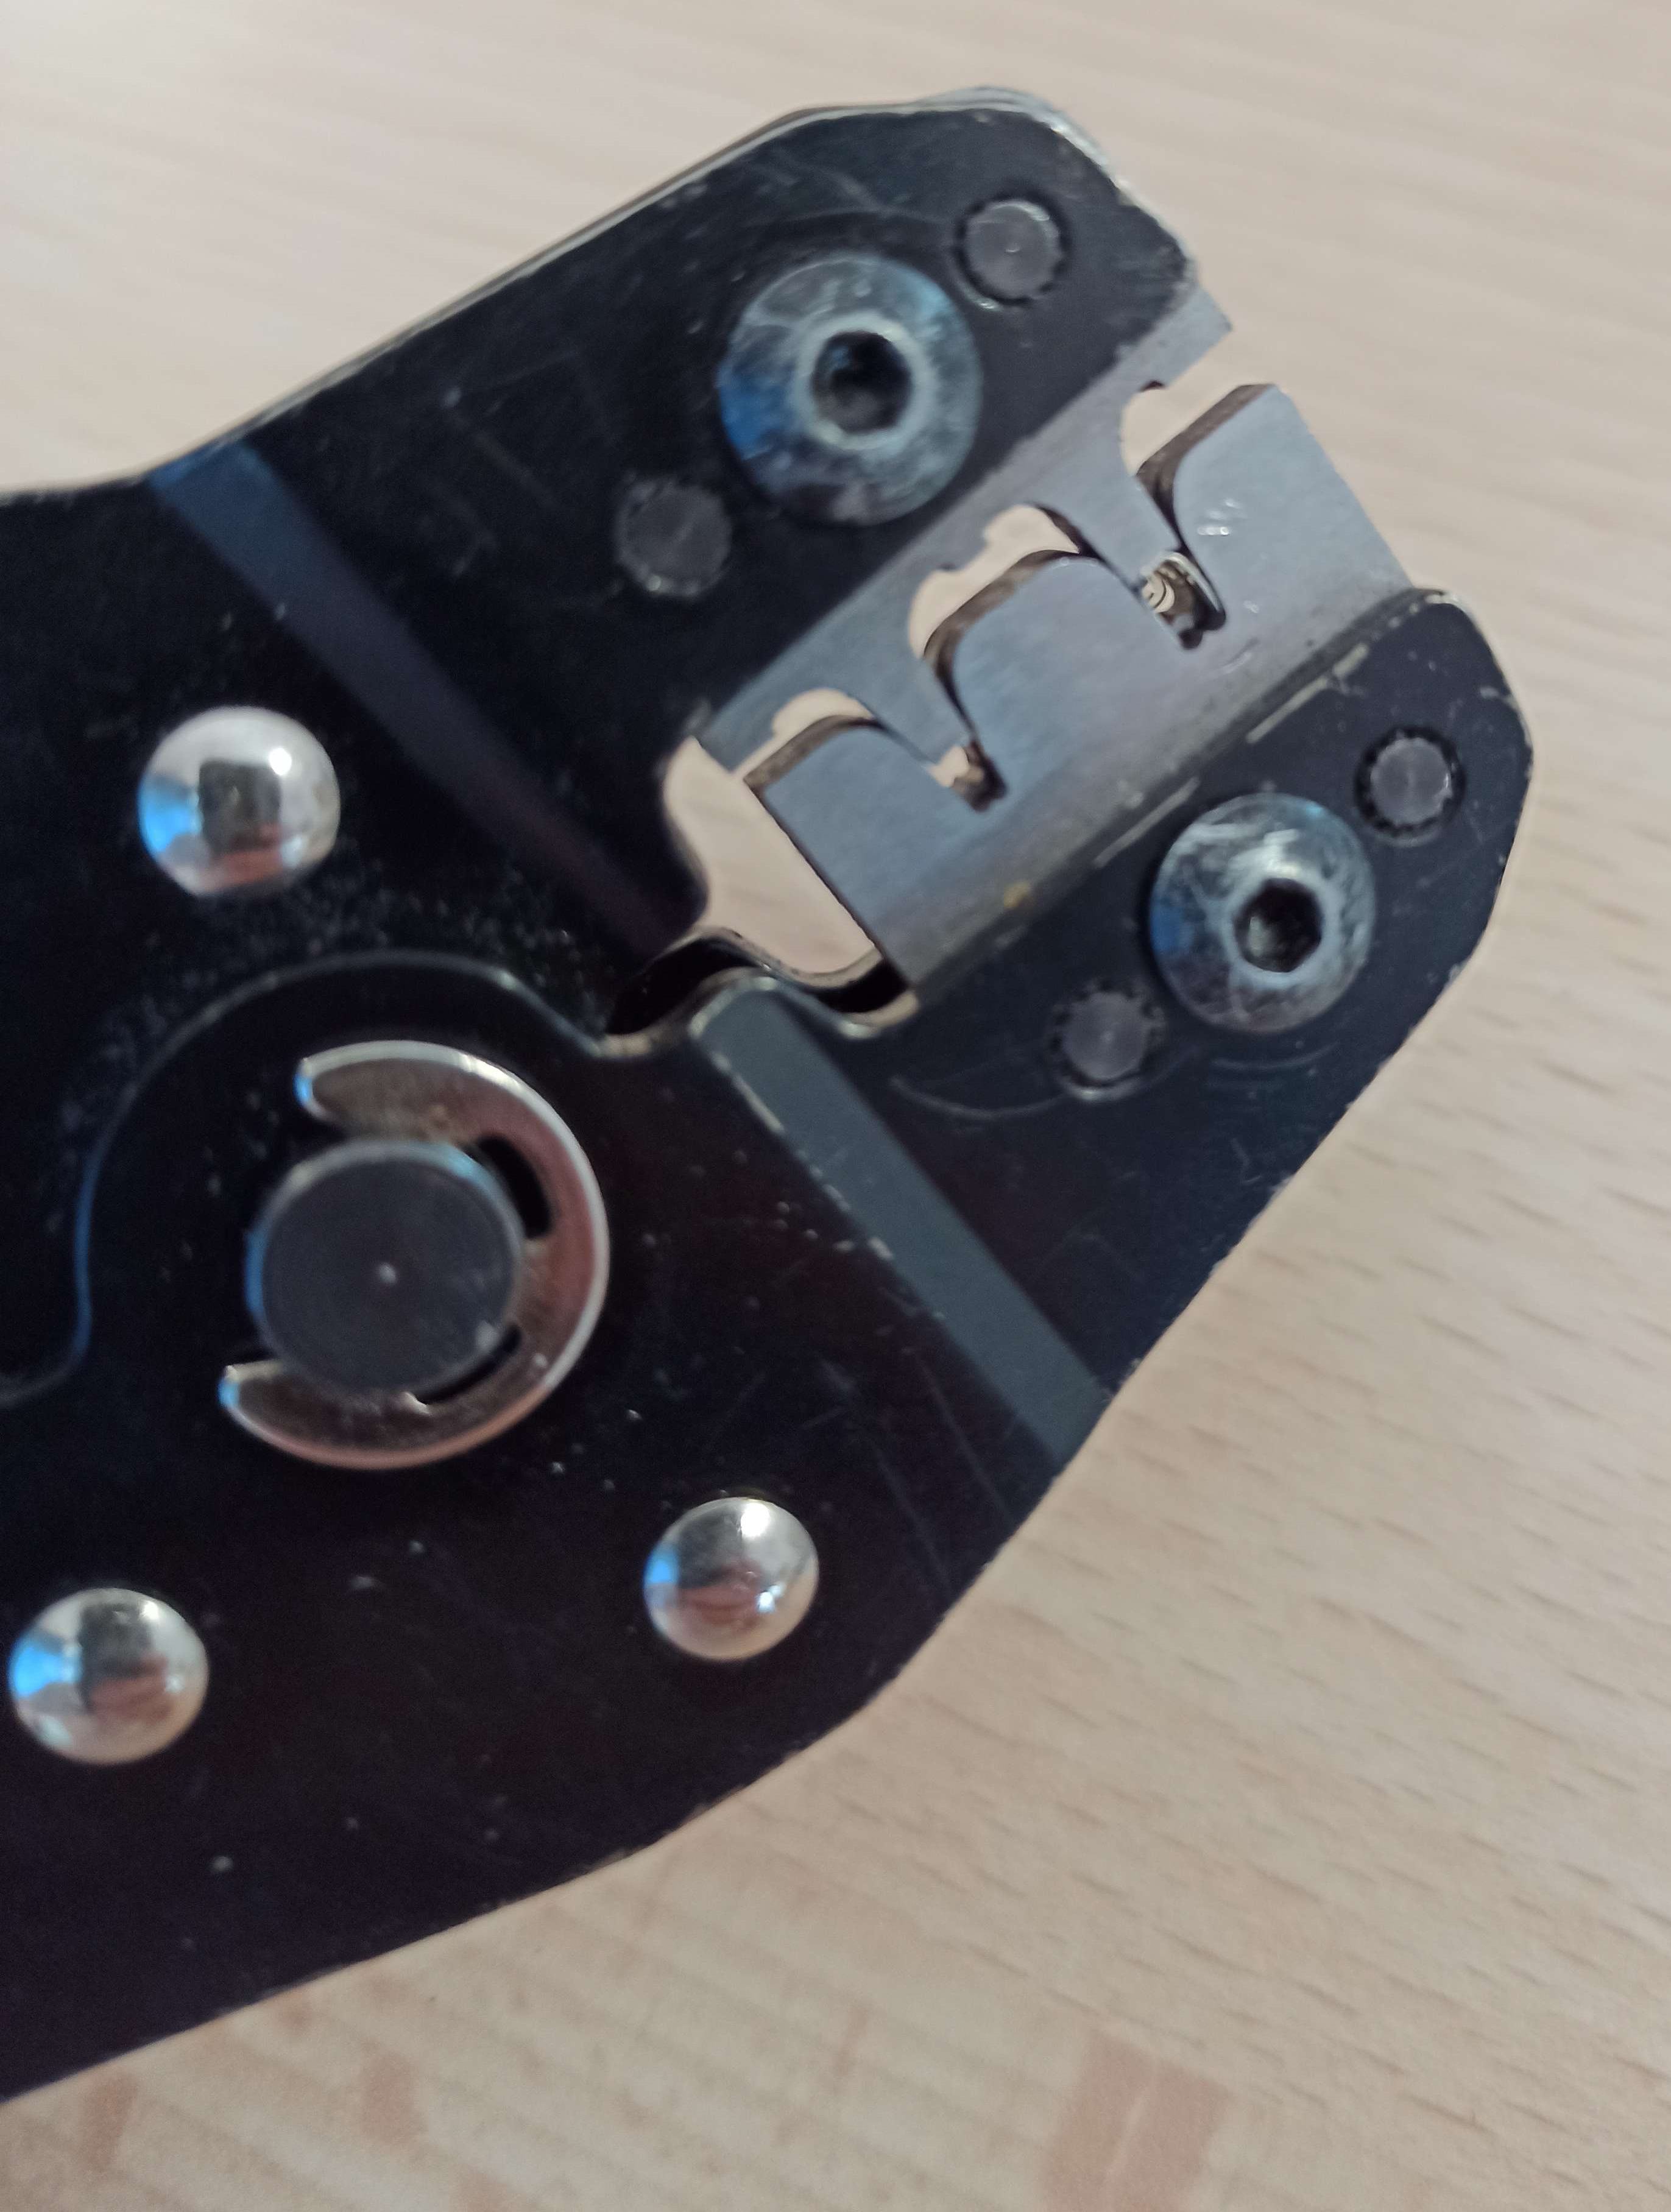
\includegraphics[width=0.4\textwidth]{images/fixer_cosse_dans_pince_sertir.jpg}
    \captionsetup{labelformat=empty}
    \captionof{figure}{}
    \end{center}
    \vspace{0.5cm}
\end{minipage}

Insérez maintenant votre fil dénudé, en l'enforçant vous allez sentir qu'il va buter à l'intérieur de la cosse, c'est normal. 

\begin{minipage}{\textwidth}
    \vspace{0.5cm}
    \begin{center}
    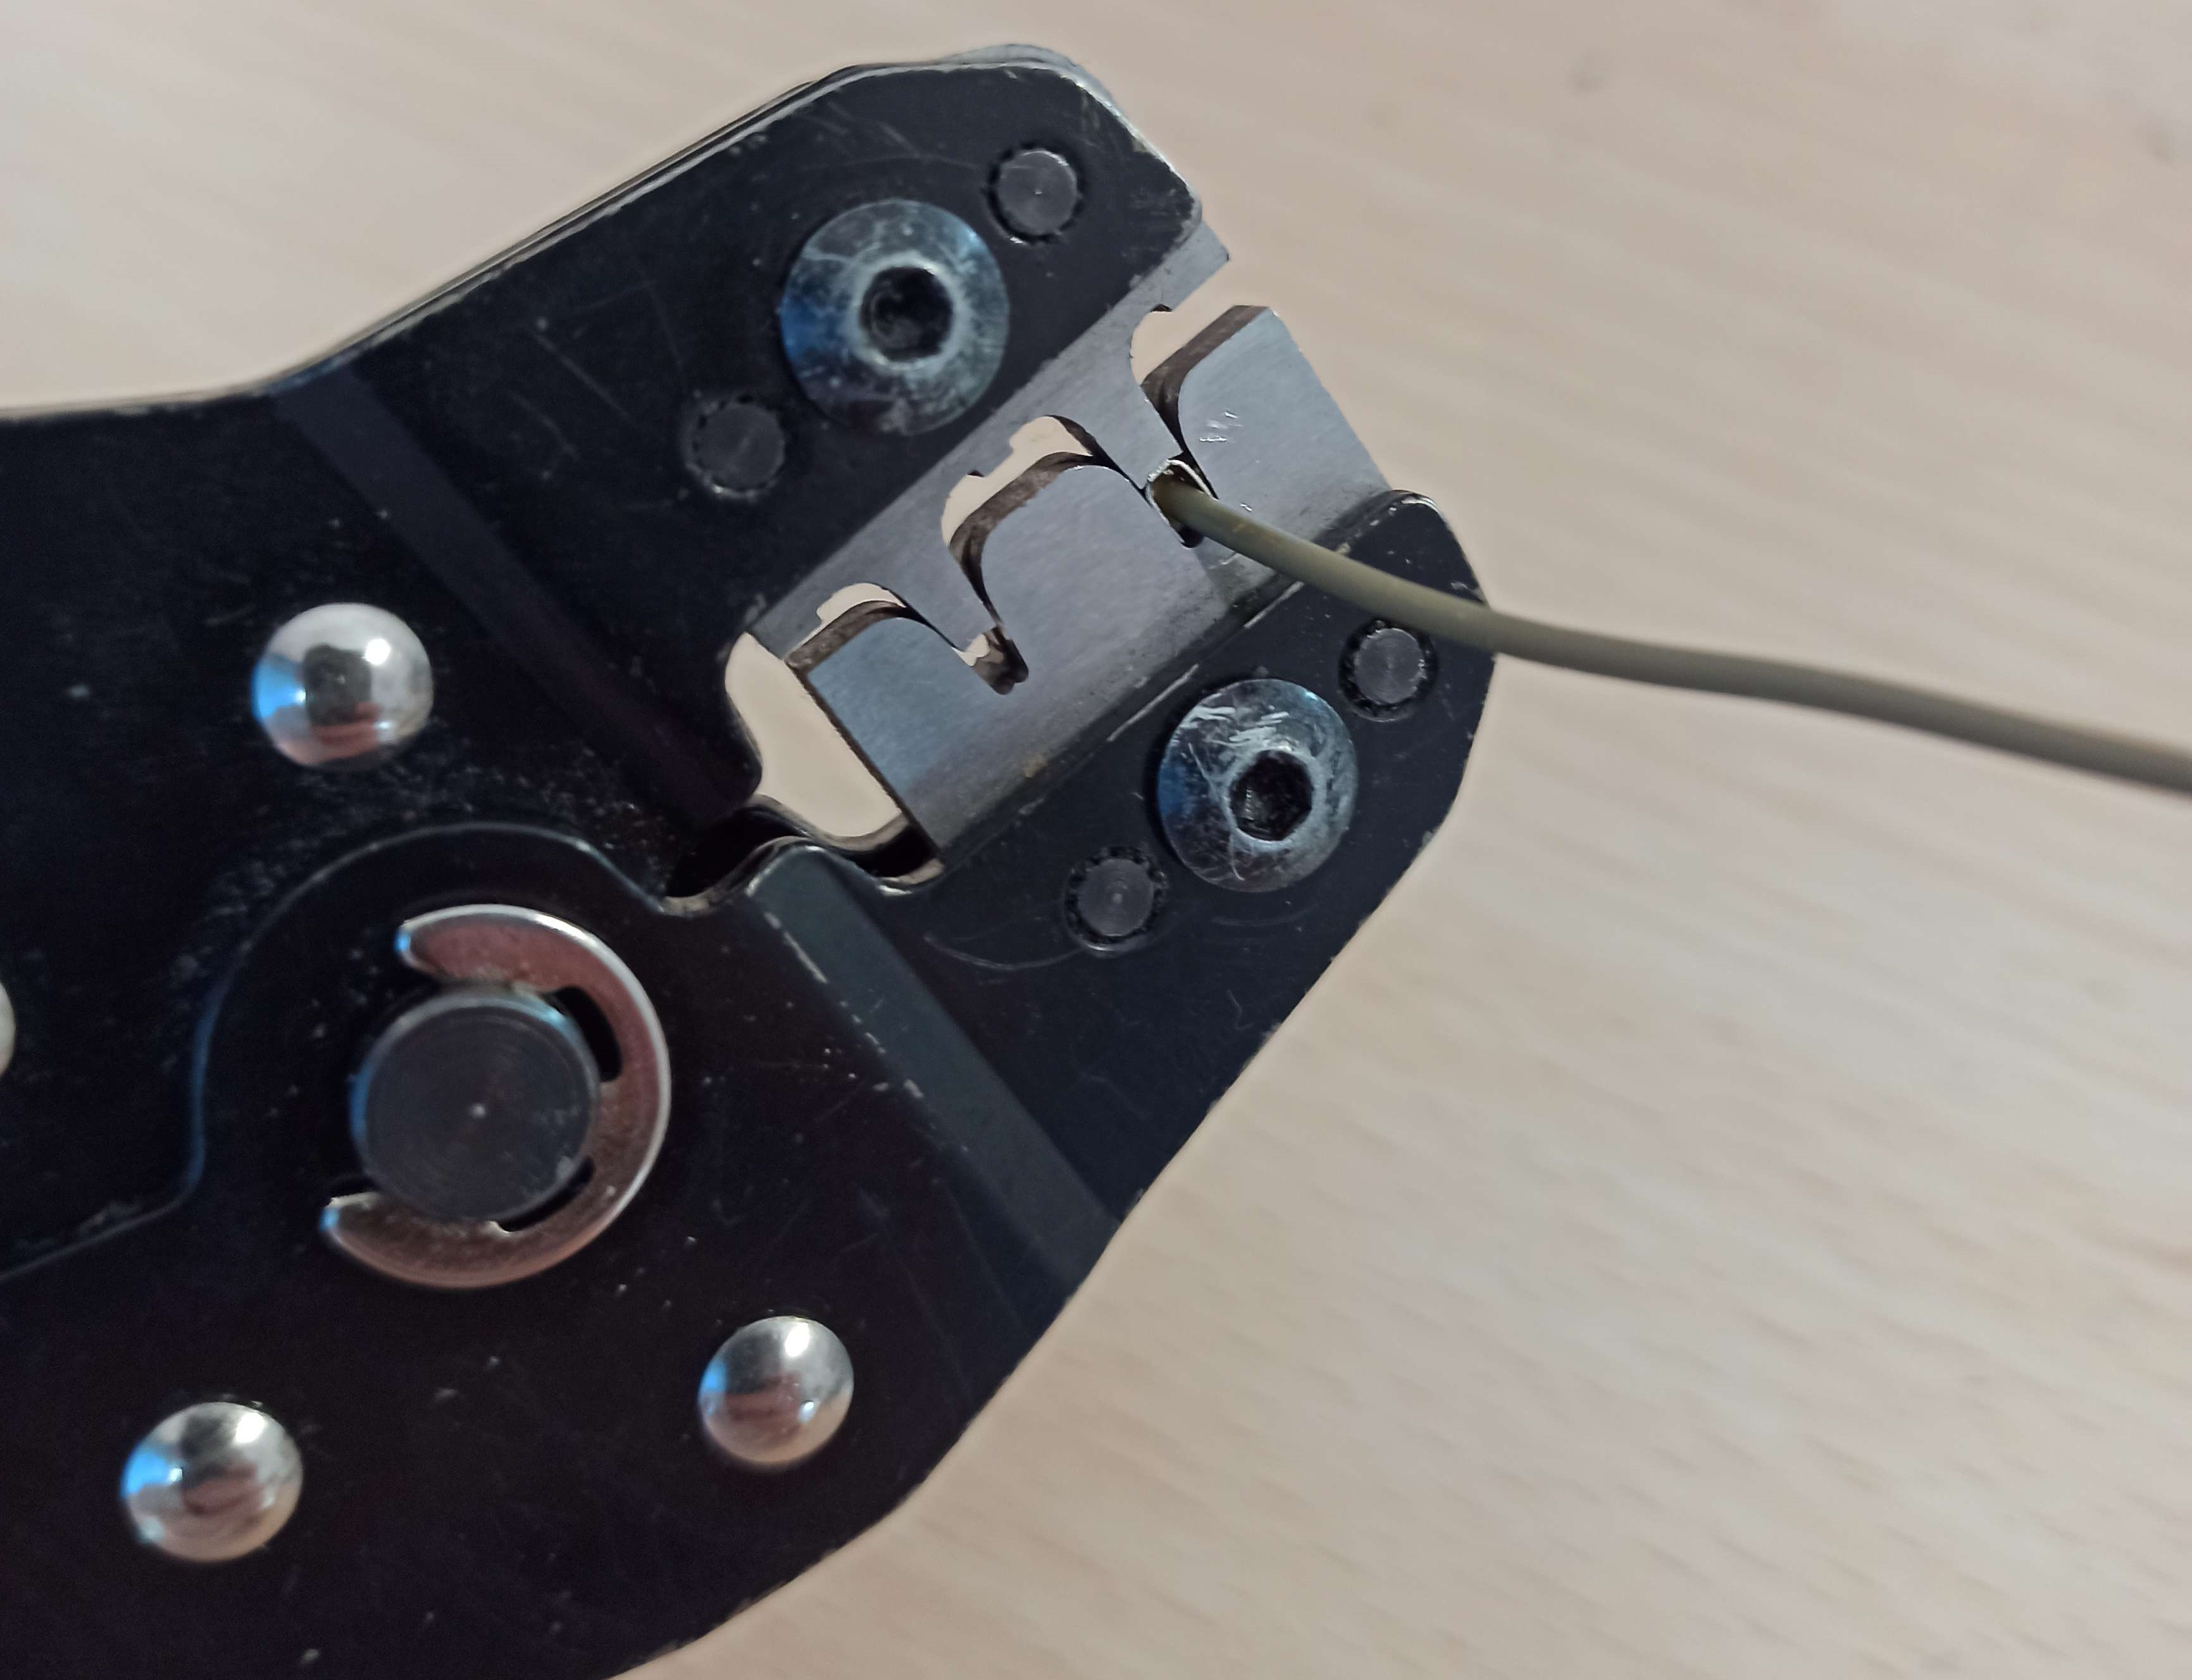
\includegraphics[width=0.4\textwidth]{images/sertissage_fil.jpg}
    \captionsetup{labelformat=empty}
    \captionof{figure}{}
    \end{center}
    \vspace{0.5cm}
\end{minipage}

Maintenant, serrez jusqu'à ce que la pince se relâche. Et voilà votre câble est sertit!

\begin{minipage}{\textwidth}
    \vspace{0.5cm}
    \begin{center}
    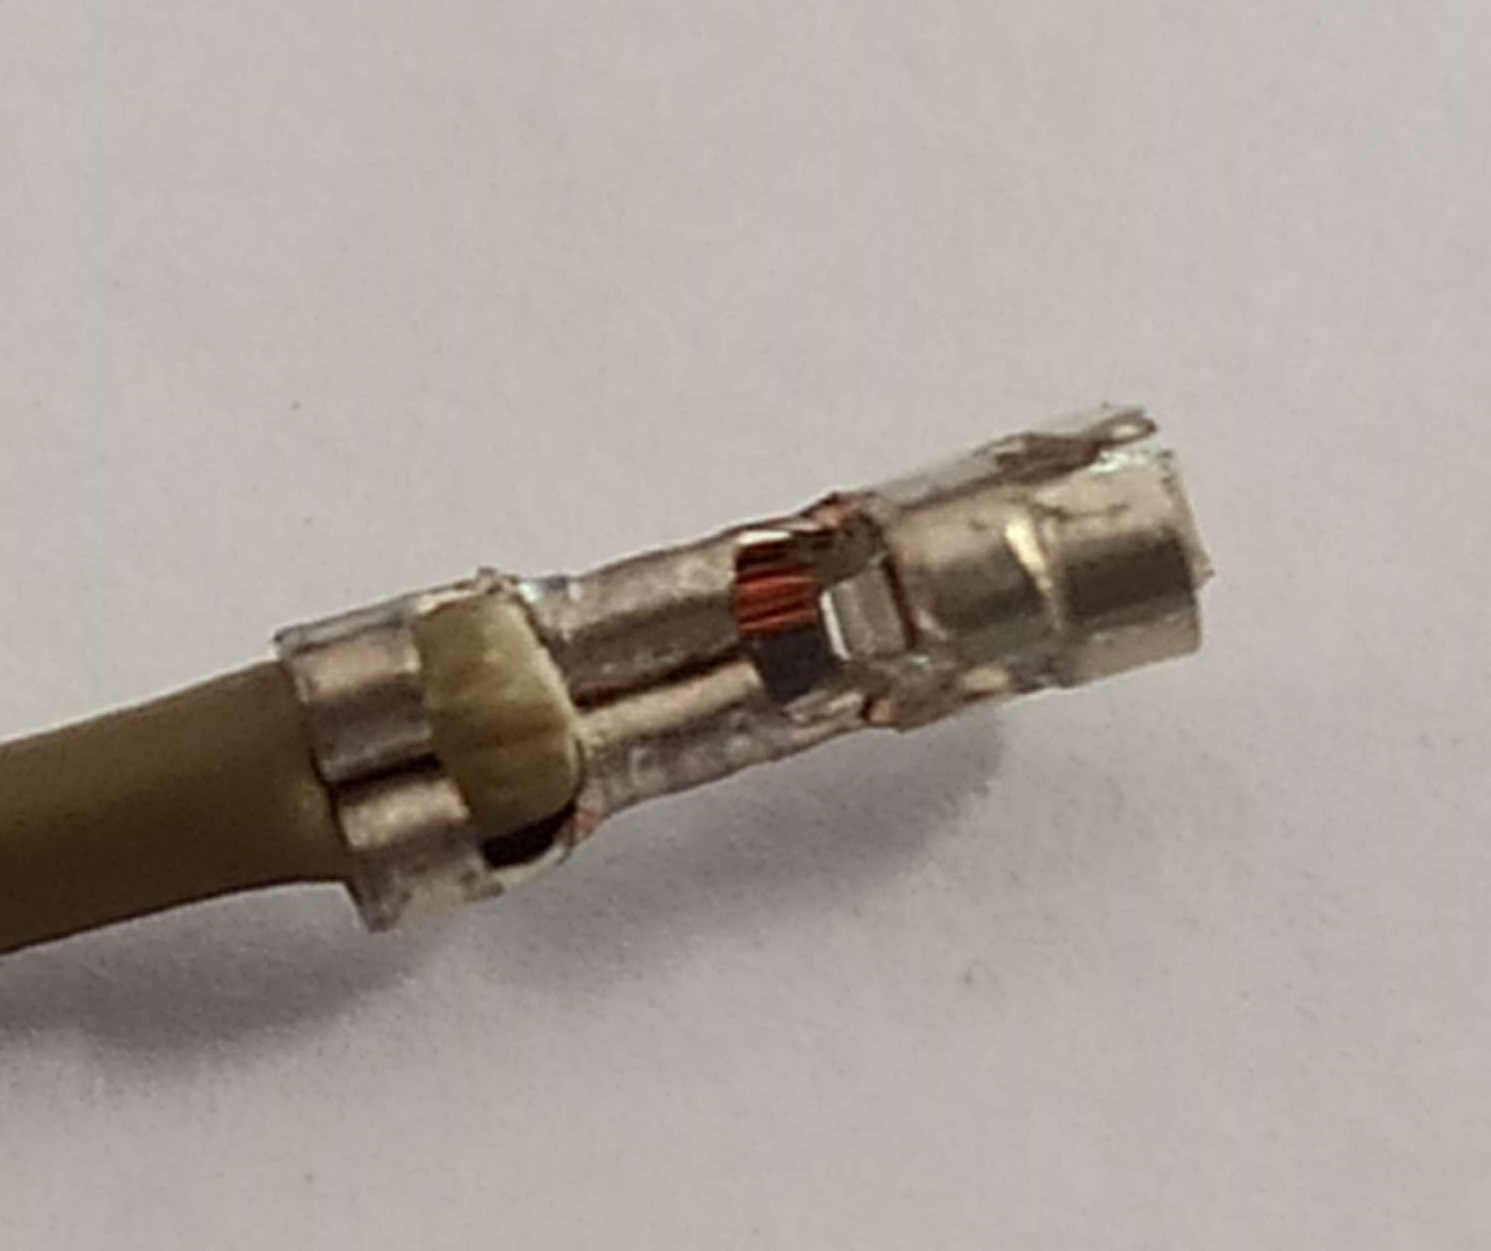
\includegraphics[width=0.4\textwidth]{images/sertissage_finit.jpg}
    \captionsetup{labelformat=empty}
    \captionof{figure}{}
    \end{center}
    \vspace{0.5cm}
\end{minipage}

\section*{Étape 3: les connecteurs JST}

Cette dernière étape est facile si le sertissage a été correctement effectué. Il faut mettre la cosse dans les connecteurs JST XH femelles. La forme de la cosse indique comment elle s'emboite dans le connecteur femelle.

\begin{figure}[h]
    \begin{minipage}{0.45\textwidth}
        \centering
        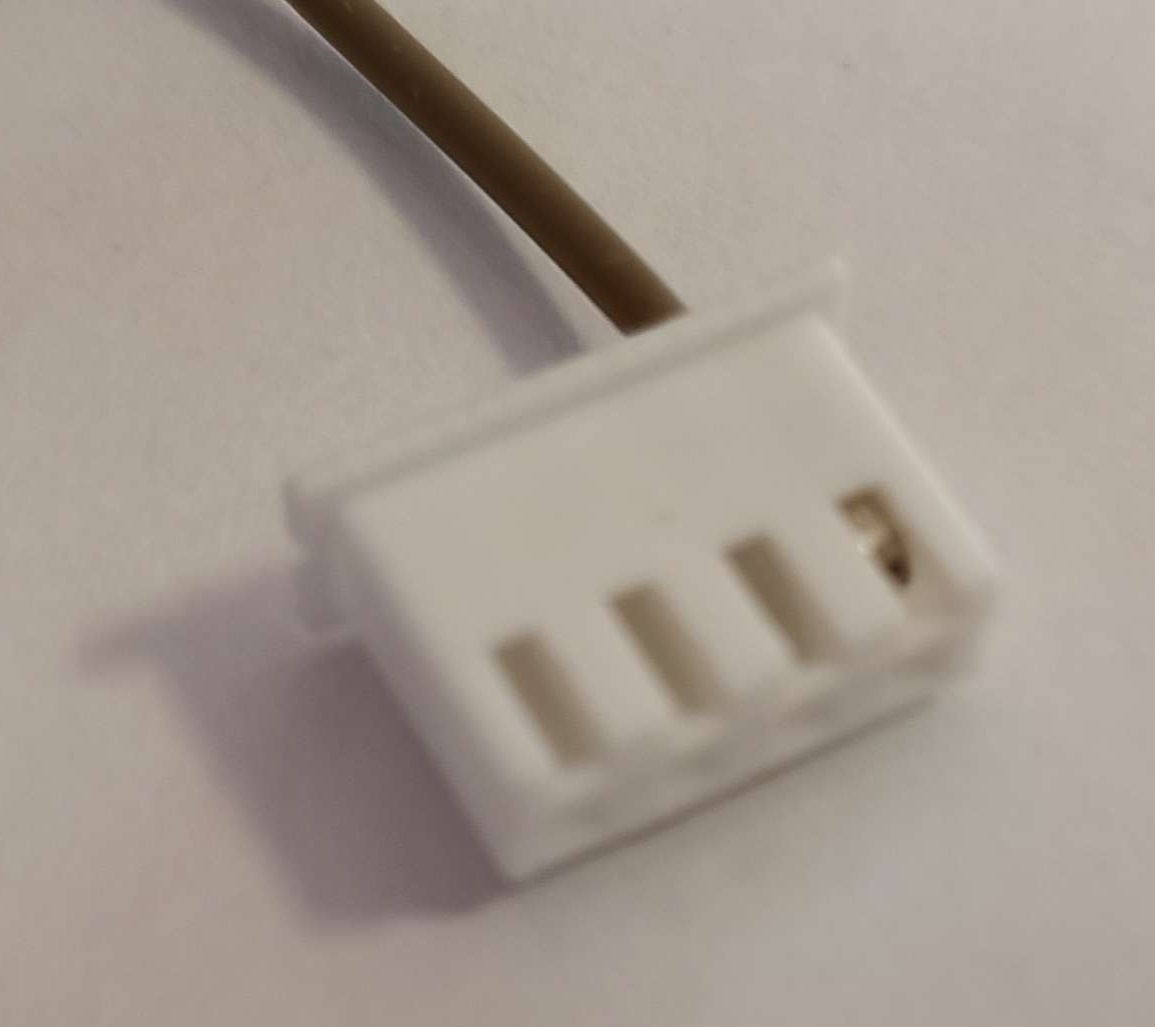
\includegraphics[width=\linewidth]{images/fil_pas_encore_totalement_enfonce_JST.jpg}
        \captionsetup{labelformat=empty}
        \caption{Fil pas encore totalement enfoncé}
        \label{fig:image1}
    \end{minipage}
    \hfill
    \begin{minipage}{0.45\textwidth}
        \centering
        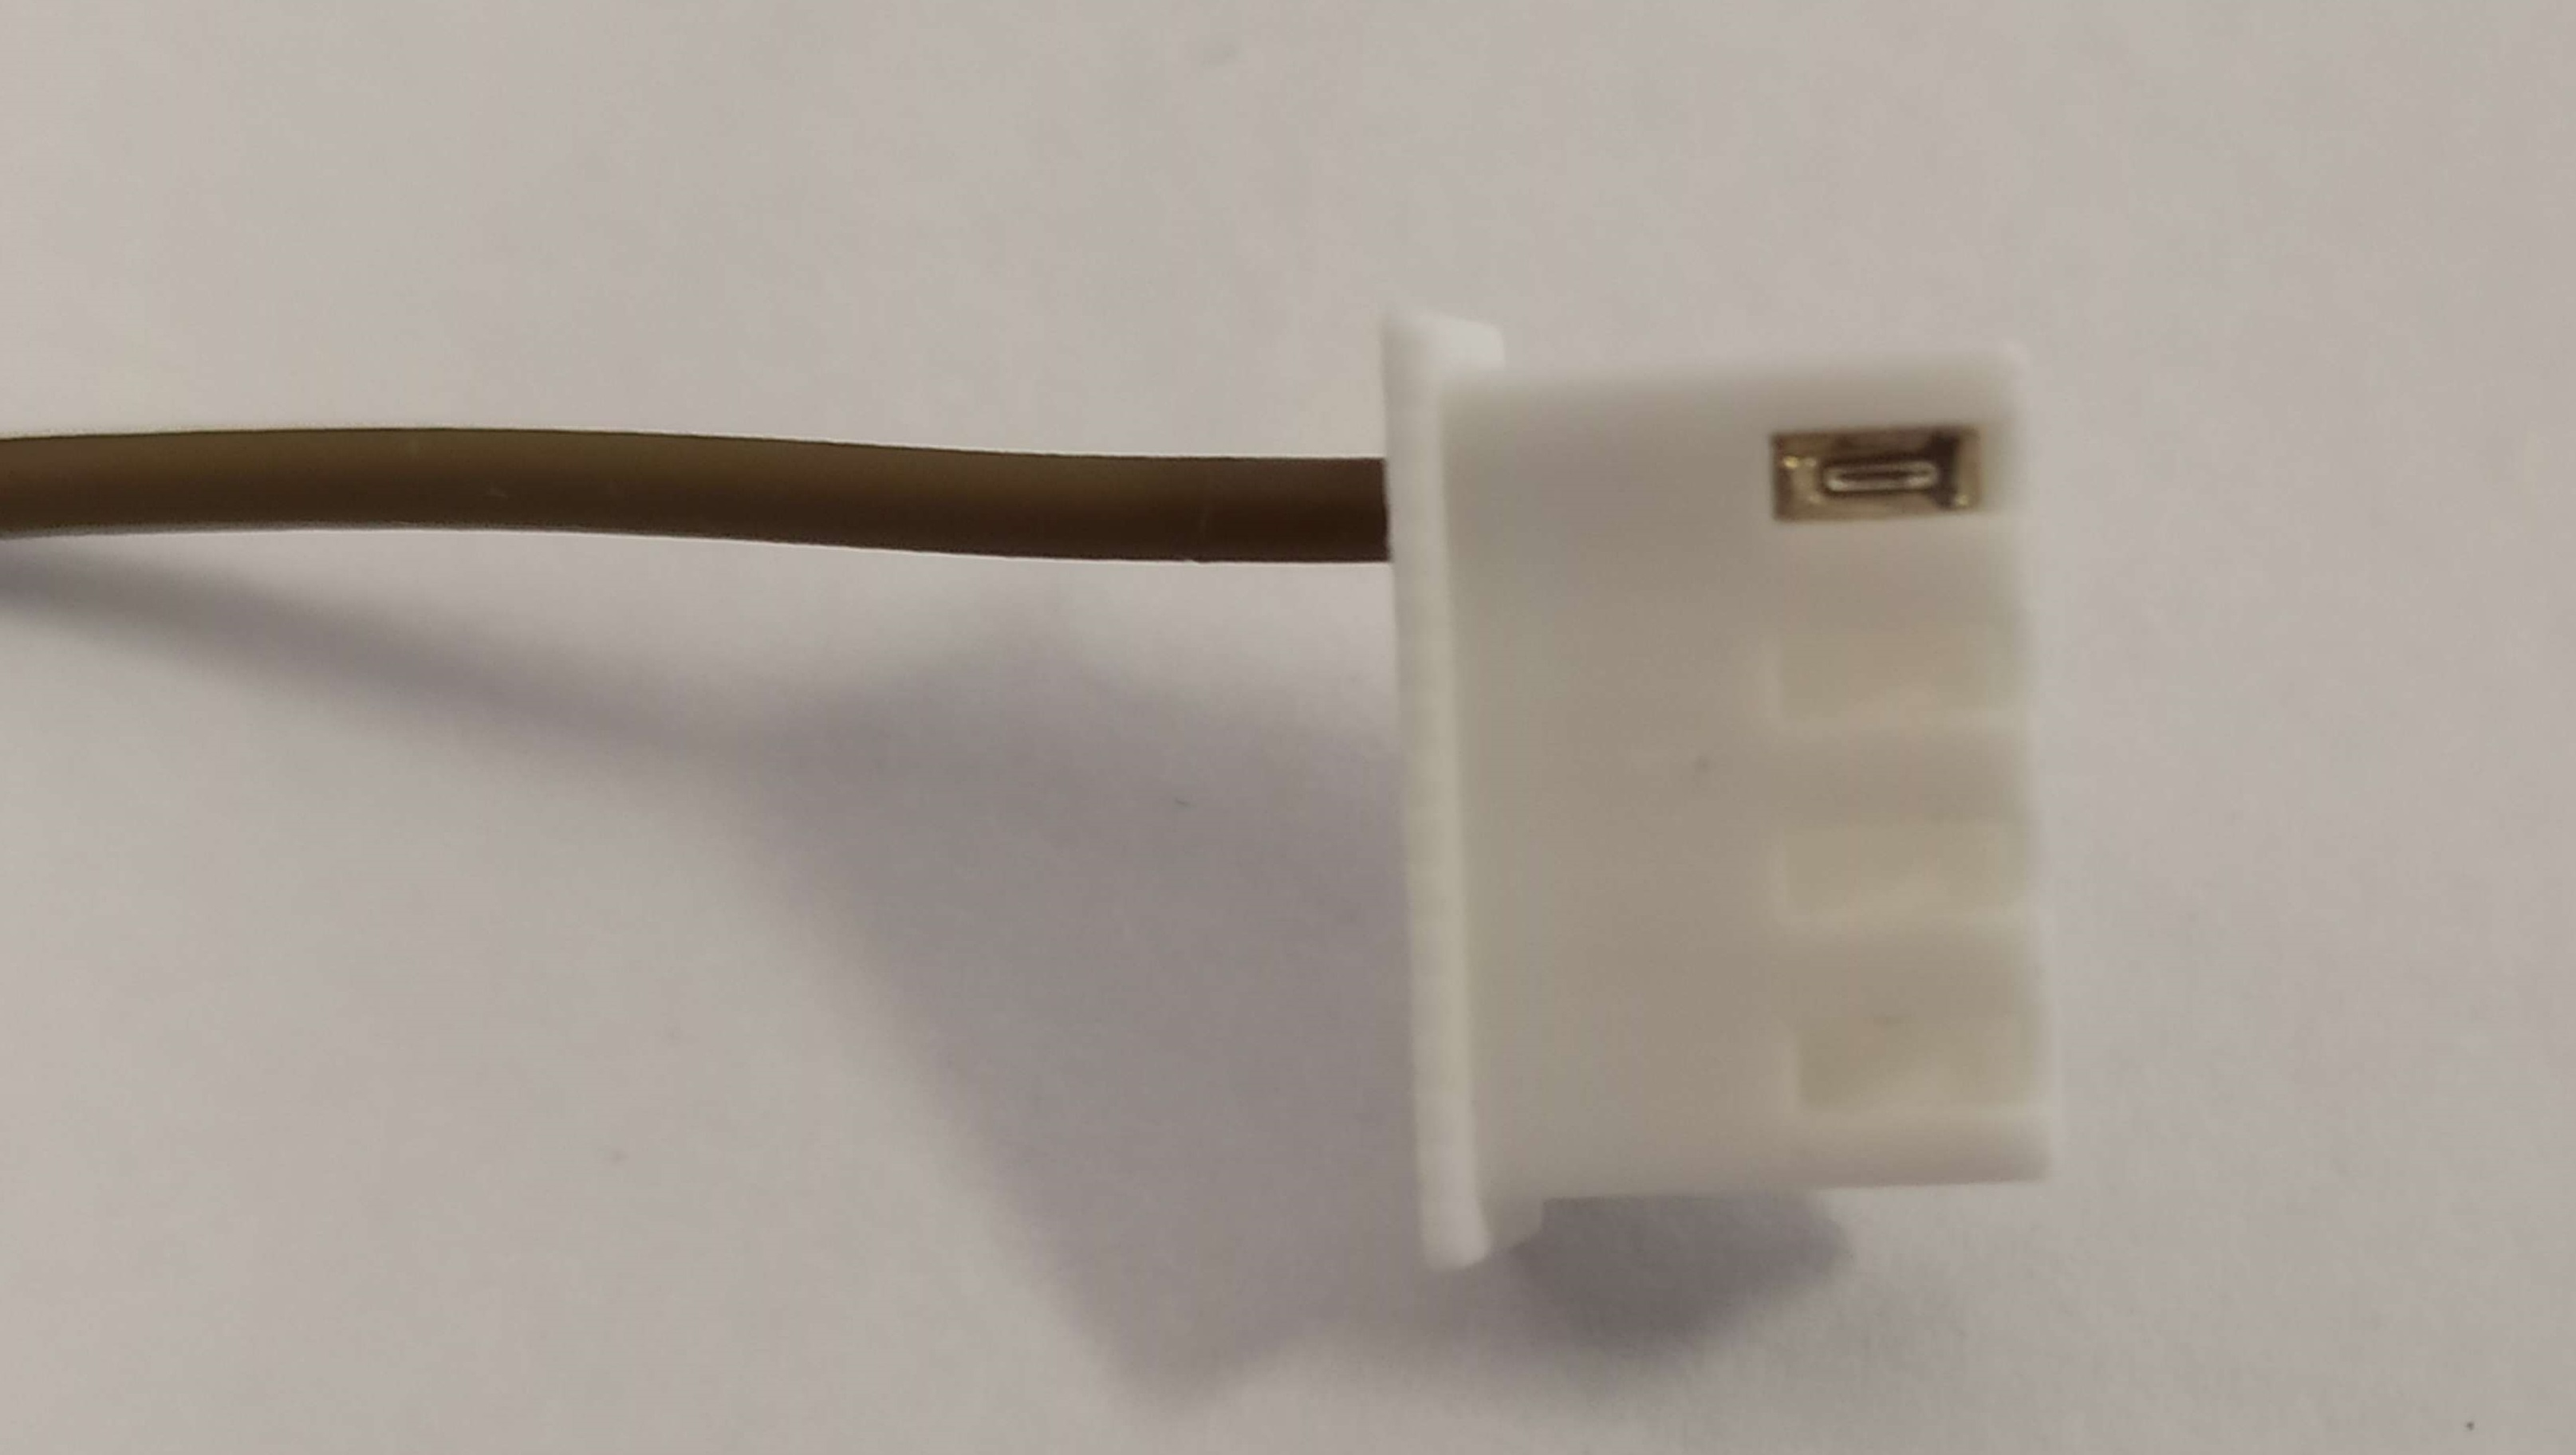
\includegraphics[width=\linewidth]{images/JST_resultat_final.jpg}
        \captionsetup{labelformat=empty}
        \caption{Fil entièrement enfoncé}
        \label{fig:image2}
    \end{minipage}
\end{figure}

\newpage
\section*{Étape 4: la vérification}

Pour vérifier que vous avez une bonne connection, c'est très simple:
\begin{itemize}
    \item déjà quand vous voyez la câble dans le connecteur, avez-vous l'impression qu'il va se casser si on le tire? 
    \item si vous tirez sur le cable et le JST, est-ce que la cosse quitte le connecteur ou le câble se rompt?
    \item si vous connectez le connecteur femelle avec le connecteur mâle, est-ce que la cosse quite le connecteur femelle?
    \item dernière vérification, contrôlez la continuité électrique du fil avec un multimètre
\end{itemize}

Et voilà vous avez une connection solide et robuste! Sinon le mieux c'est de recommencer tout depuis l'étape 1. Par expérience, laisser un mauvais sertissage dans un câblage provoquera toujours des problèmes tôt ou tard et ce n'est que partie remise.

\end{document}
